\documentclass[11pt]{article}

\usepackage{amsmath,amssymb,amsfonts}
\usepackage{graphicx}
\usepackage{booktabs}
\usepackage{geometry}
\usepackage{float}
\usepackage{caption}
\usepackage{subcaption}
\usepackage{hyperref}
\usepackage{enumitem}

\geometry{margin=1in}

\title{
Residual Manifold Operators:\\
Transport Geometry, Spectral Hierarchy,
and Topology-Family Continuity
}

\author{
Dan Hawkley\\
Boulder, Colorado\\
\url{https://github.com/thinkthoughts/residue-manifold-learning}
}

\date{2026}

\begin{document}

\maketitle

\begin{abstract}

Residual manifold operators provide a geometric framework for studying continuity structure across graph topology families. We construct residual manifolds from topology-conditioned graph embeddings and evaluate how density reconstruction, geodesic transport, diffusion persistence, and Laplacian spectral operators preserve topology-family organization under graph scaling.

Residual density operators produce topology-localized support regions with stable family separation across graph size transitions. Geodesic transport operators preserve manifold adjacency structure while bridgeability matrices reveal asymmetric transport accessibility between topology families. Diffusion persistence operators retain topology-local neighborhoods under iterative propagation, while Laplacian spectral decompositions expose cumulative eigengap hierarchies, topology-family overlap structure, and spectral regime transitions.

Residual spectral organization separates into continuity-preserving, transport-coupling, and fragmentation-dominant operator regimes. Spectral trajectories evolve continuously across graph scaling while preserving cross-family separability throughout residual spectral space.

The resulting operator hierarchy demonstrates that residual manifold organization remains stable across density, transport, diffusion, and spectral measurements simultaneously.

\end{abstract}

\section{Introduction}

Residual manifold geometry provides a structured framework for evaluating continuity relationships across graph topology families. Spectral graph operators, diffusion geometry, and manifold embeddings provide natural mathematical foundations for studying continuity structure across graph topology systems \cite{chung1997spectral,coifman2006diffusion,belkin2003laplacian}. Rather than treating graph embeddings as isolated coordinate systems, residual manifold operators evaluate how topology-conditioned structure persists under density reconstruction, geodesic transport structure, diffusion propagation, and spectral decomposition.

This work studies five graph topology families:

\begin{itemize}
\item ring lattice,
\item small world,
\item Erd\H{o}s--R\'enyi,
\item scale free,
\item modular clustered.
\end{itemize}

These topology constructions correspond to classical random-graph and network-organization models developed across graph theory and network science \cite{erdos1959random,watts1998collective,barabasi1999emergence}.

Each family is evaluated across graph scaling parameters:
\[
N \in \{16,32,64,128\}.
\]

Residual manifold operators are then constructed over the resulting embedding geometry.

The paper develops a coupled residual operator hierarchy spanning:

\begin{enumerate}
\item residual density operators,
\item geodesic transport operators,
\item diffusion persistence operators,
\item Laplacian spectral operators.
\end{enumerate}

Across all measured operators, family-level operator structure remains stable under graph scaling while resisting cross-family residual collapse and spectral mixing.

\begin{figure}[H]
\centering
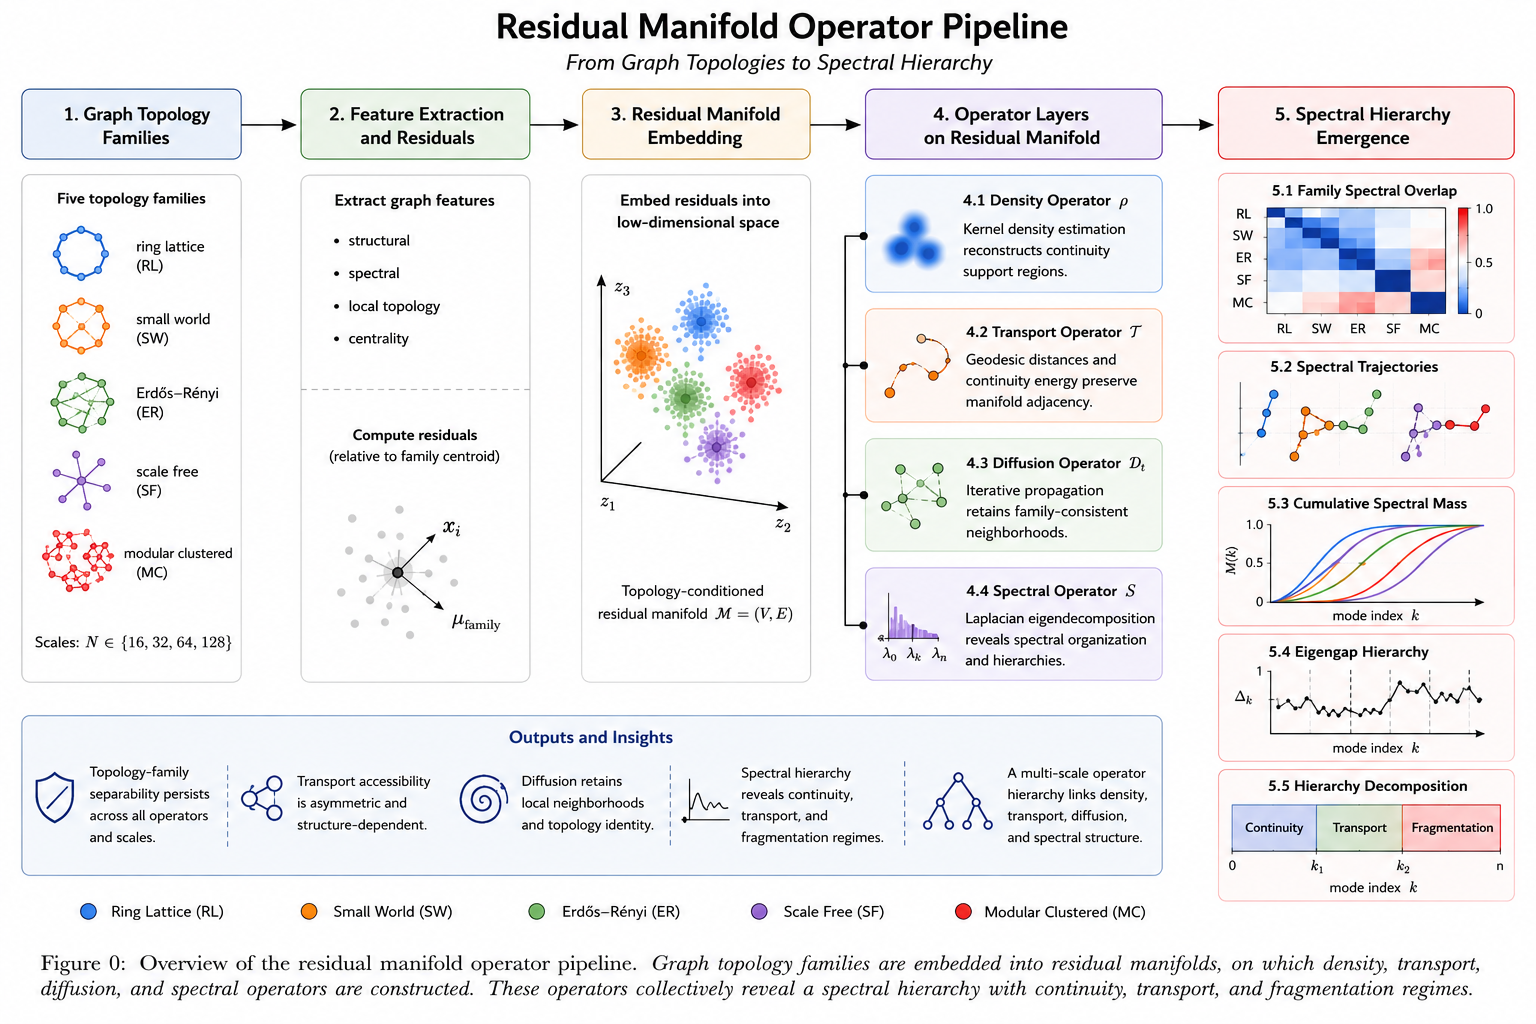
\includegraphics[width=\textwidth]{figures/00_residual_manifold_operator_pipeline.png}
\caption{
Overview of the residual manifold operator pipeline. Graph topology families are embedded into residual manifolds, on which density, transport, diffusion, and spectral operators are constructed. These operators collectively reveal a spectral hierarchy with continuity, transport, and fragmentation regimes.
}
\label{fig:operator_pipeline}
\end{figure}

\section{Residual Operators}

Let residual manifold coordinates be denoted:
\[
x_i \in \mathbb{R}^d.
\]

Residual continuity operators are constructed over topology-family neighborhoods embedded within residual coordinate space.

We define:
\[
\mathcal{M}=(V,E)
\]
where \(V\) represents residual manifold coordinates and \(E\) represents continuity-preserving neighborhood relations.

Residual manifolds are topology-conditioned embedding geometries constructed from graph-family feature residuals across graph scaling.

Residual operators are evaluated across:

\begin{itemize}
\item density continuity,
\item nearest-family structure,
\item geodesic transport,
\item diffusion persistence,
\item Laplacian spectral decomposition.
\end{itemize}

Residual operator mappings may therefore be represented:

\[
\rho : \mathcal{M} \rightarrow \mathbb{R}
\]

\[
\mathcal{T} : \mathcal{M} \rightarrow \mathcal{M}
\]

\[
\mathcal{D}_t : \mathcal{M} \rightarrow \mathcal{M}
\]

\[
\mathcal{S} : \mathcal{M} \rightarrow \Lambda
\]

corresponding respectively to density reconstruction, transport flow, diffusion evolution, and spectral projection.

\section{Residual Manifold Construction}

Each topology family produces graph embeddings parameterized by graph scale \(N\).

Residual coordinates are projected into low-dimensional manifold space through topology-conditioned feature extraction.

Figure~\ref{fig:density_manifold} shows the resulting residual manifold organization.

\begin{figure}[H]
\centering
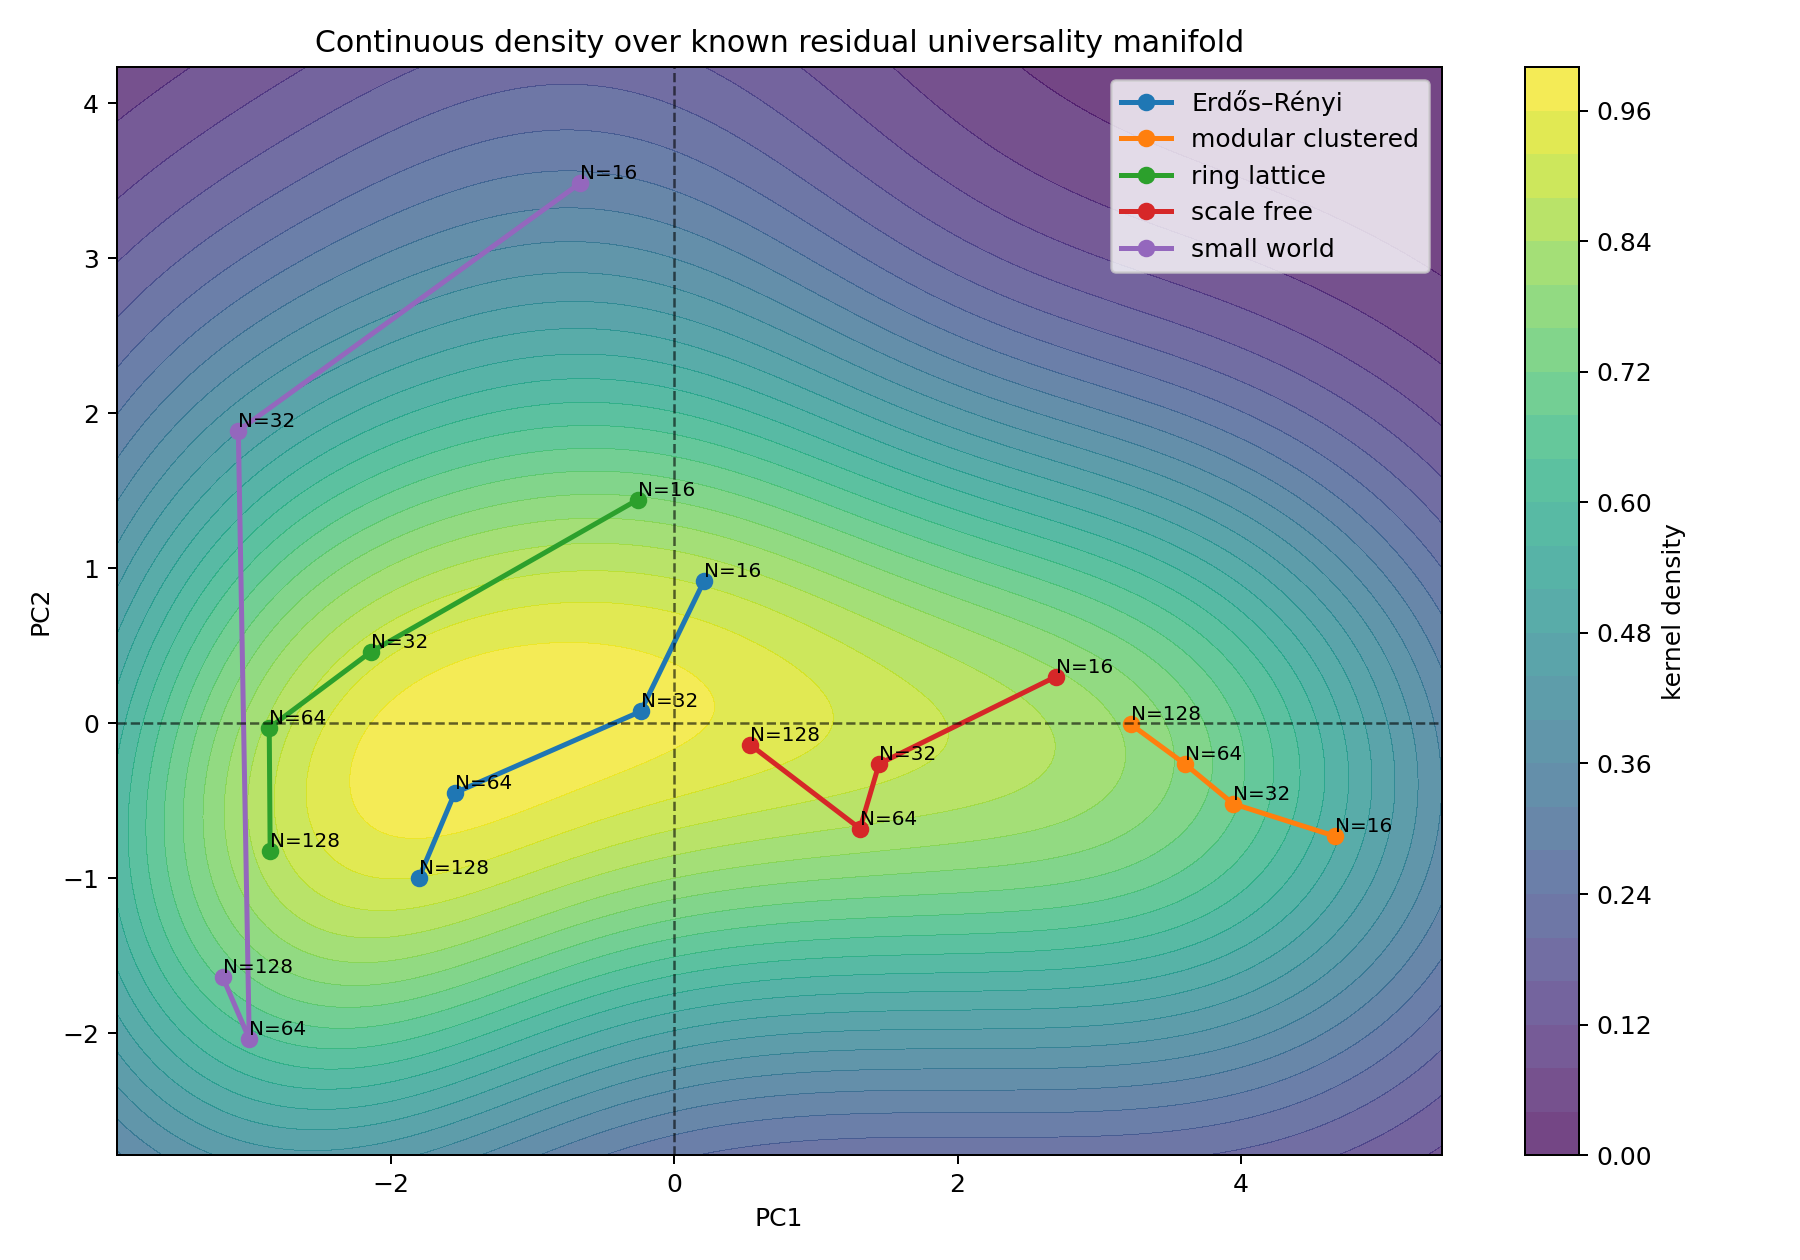
\includegraphics[width=0.82\textwidth]{figures/24_density_known_manifold.png}
\caption{
Residual manifold density structure across topology families. Distinct topology families remain geometrically separated while preserving graph scaling continuity. Density maxima remain topology-localized across residual manifold space.
}
\label{fig:density_manifold}
\end{figure}

Topology-family support regions remain non-overlapping while graph scaling trajectories evolve continuously within family-specific neighborhoods.

\section{Residual Density Geometry}

Residual density operators reconstruct topology-family continuity regions across manifold space.

Residual density is defined:
\[
\rho(x)
=
\sum_i
K\!\left(
\frac{\|x-x_i\|}{h}
\right)
\]
where \(K\) denotes a local continuity kernel and \(h\) denotes kernel bandwidth.

Density reconstruction reveals:

\begin{itemize}
\item localized family support regions,
\item stable local neighborhoods,
\item graph-scale persistence,
\item topology-family separability.
\end{itemize}

Residual density peaks preserve family ordering across manifold space while resisting cross-family residual collapse under scaling transitions.

\section{Nearest-Family Decision Geometry}

Nearest-family operators classify residual manifold regions according to local manifold structure.

Figure~\ref{fig:decision_field} shows nearest-family partition structure.

\begin{figure}[H]
\centering
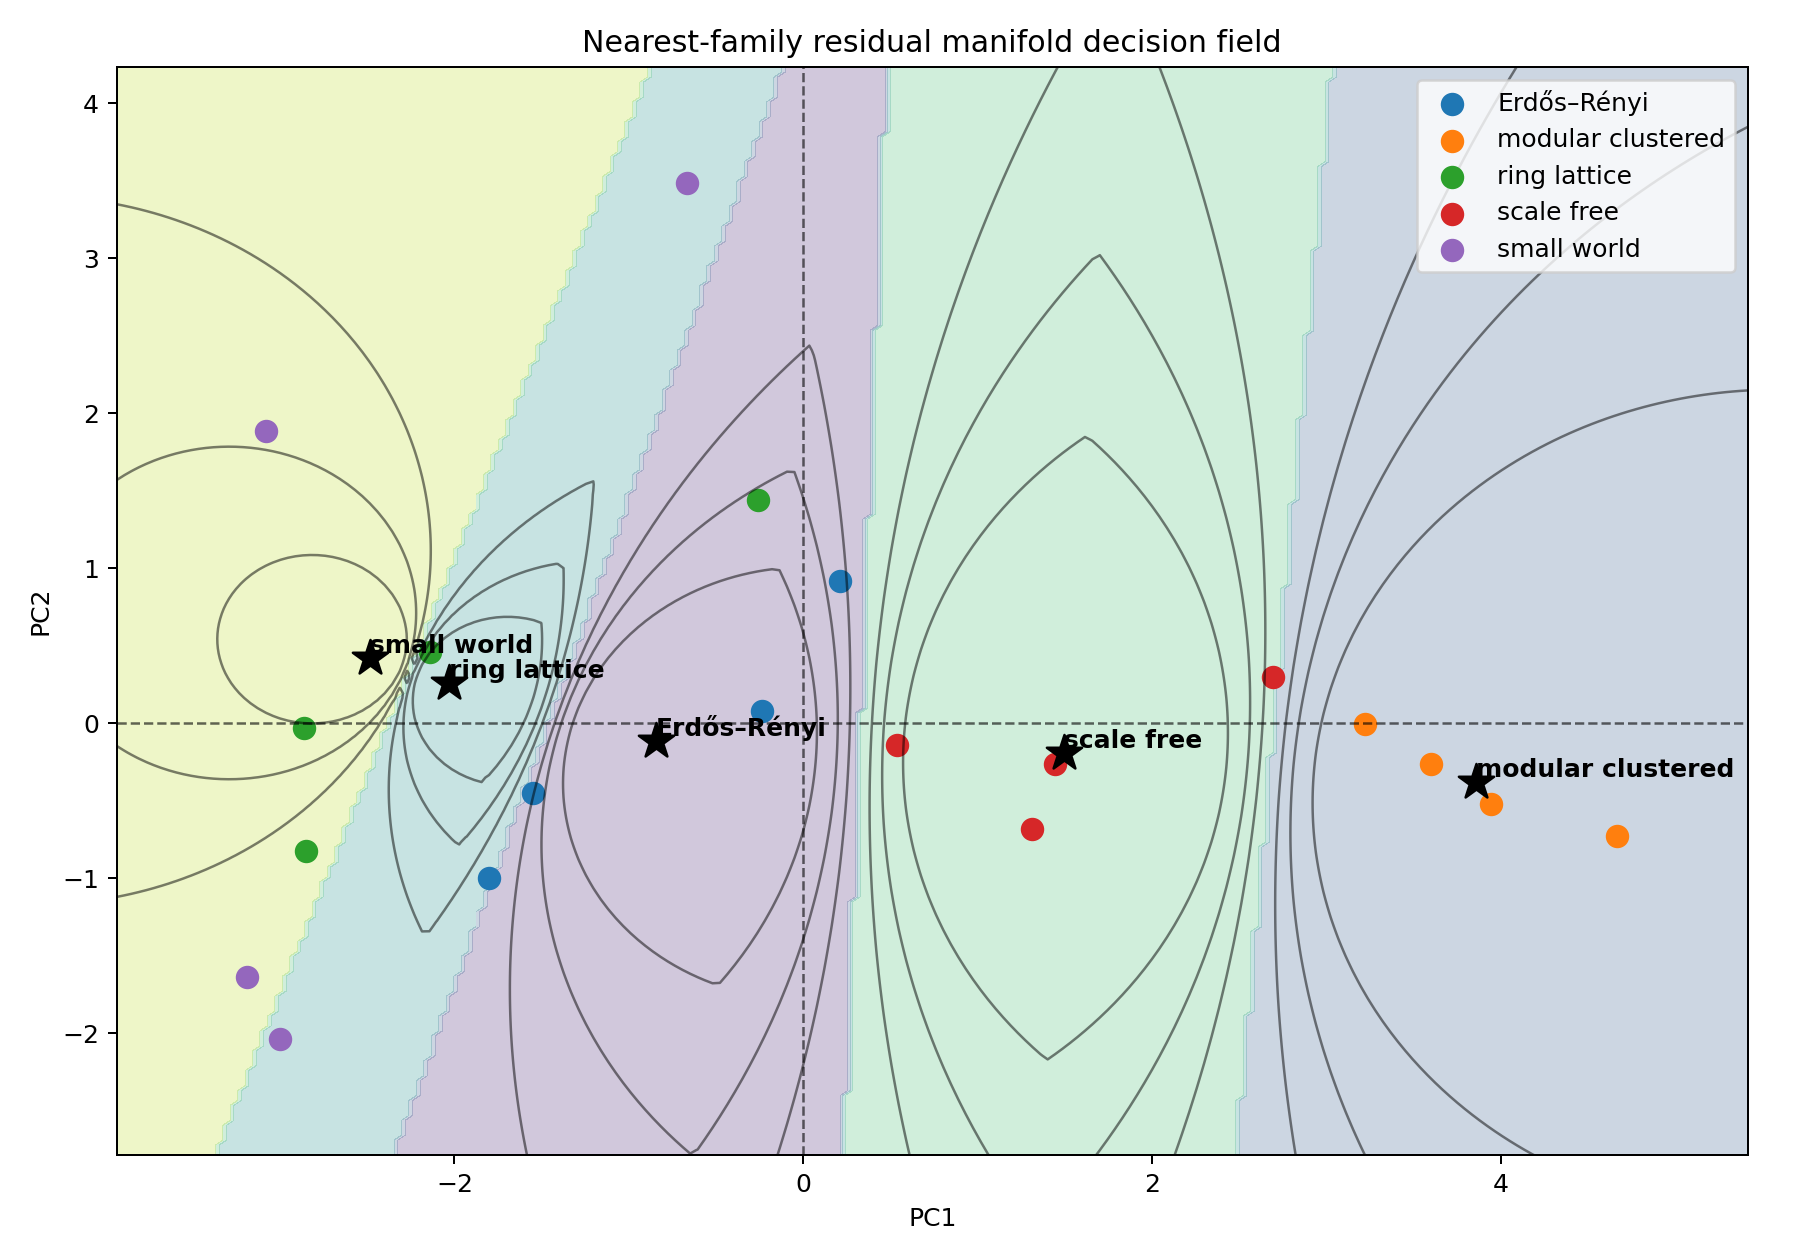
\includegraphics[width=0.78\textwidth]{figures/24_decision_field_nearest_family.png}
\caption{
Nearest-family residual manifold decision regions. Topology-family continuity domains remain geometrically separated while preserving stable family boundaries across manifold space.
}
\label{fig:decision_field}
\end{figure}

Nearest-family operators preserve local topology-family neighborhood structure while maintaining stable regional organization.

\section{Residual Transport Structure}

Residual geodesic transport operators evaluate continuity pathways between topology-family regions.

Geodesic transport distance is defined:
\[
d_g(x_i,x_j)
=
\inf_{\gamma}
\int_\gamma
\|\dot{\gamma}(t)\|dt.
\]

Geodesic transport constructions are closely related to broader optimal transport and manifold geodesic frameworks \cite{villani2008optimal}.

Continuity energy across manifold neighborhoods is defined:
\[
E_{\mathrm{cont}}
=
\sum_{(i,j)\in E}
w_{ij}
\|x_i-x_j\|^2
\]

where low continuity energy corresponds to stable coherent manifold transport organization.

Figure~\ref{fig:transport_paths} shows transport continuity pathways.

\begin{figure}[H]
\centering
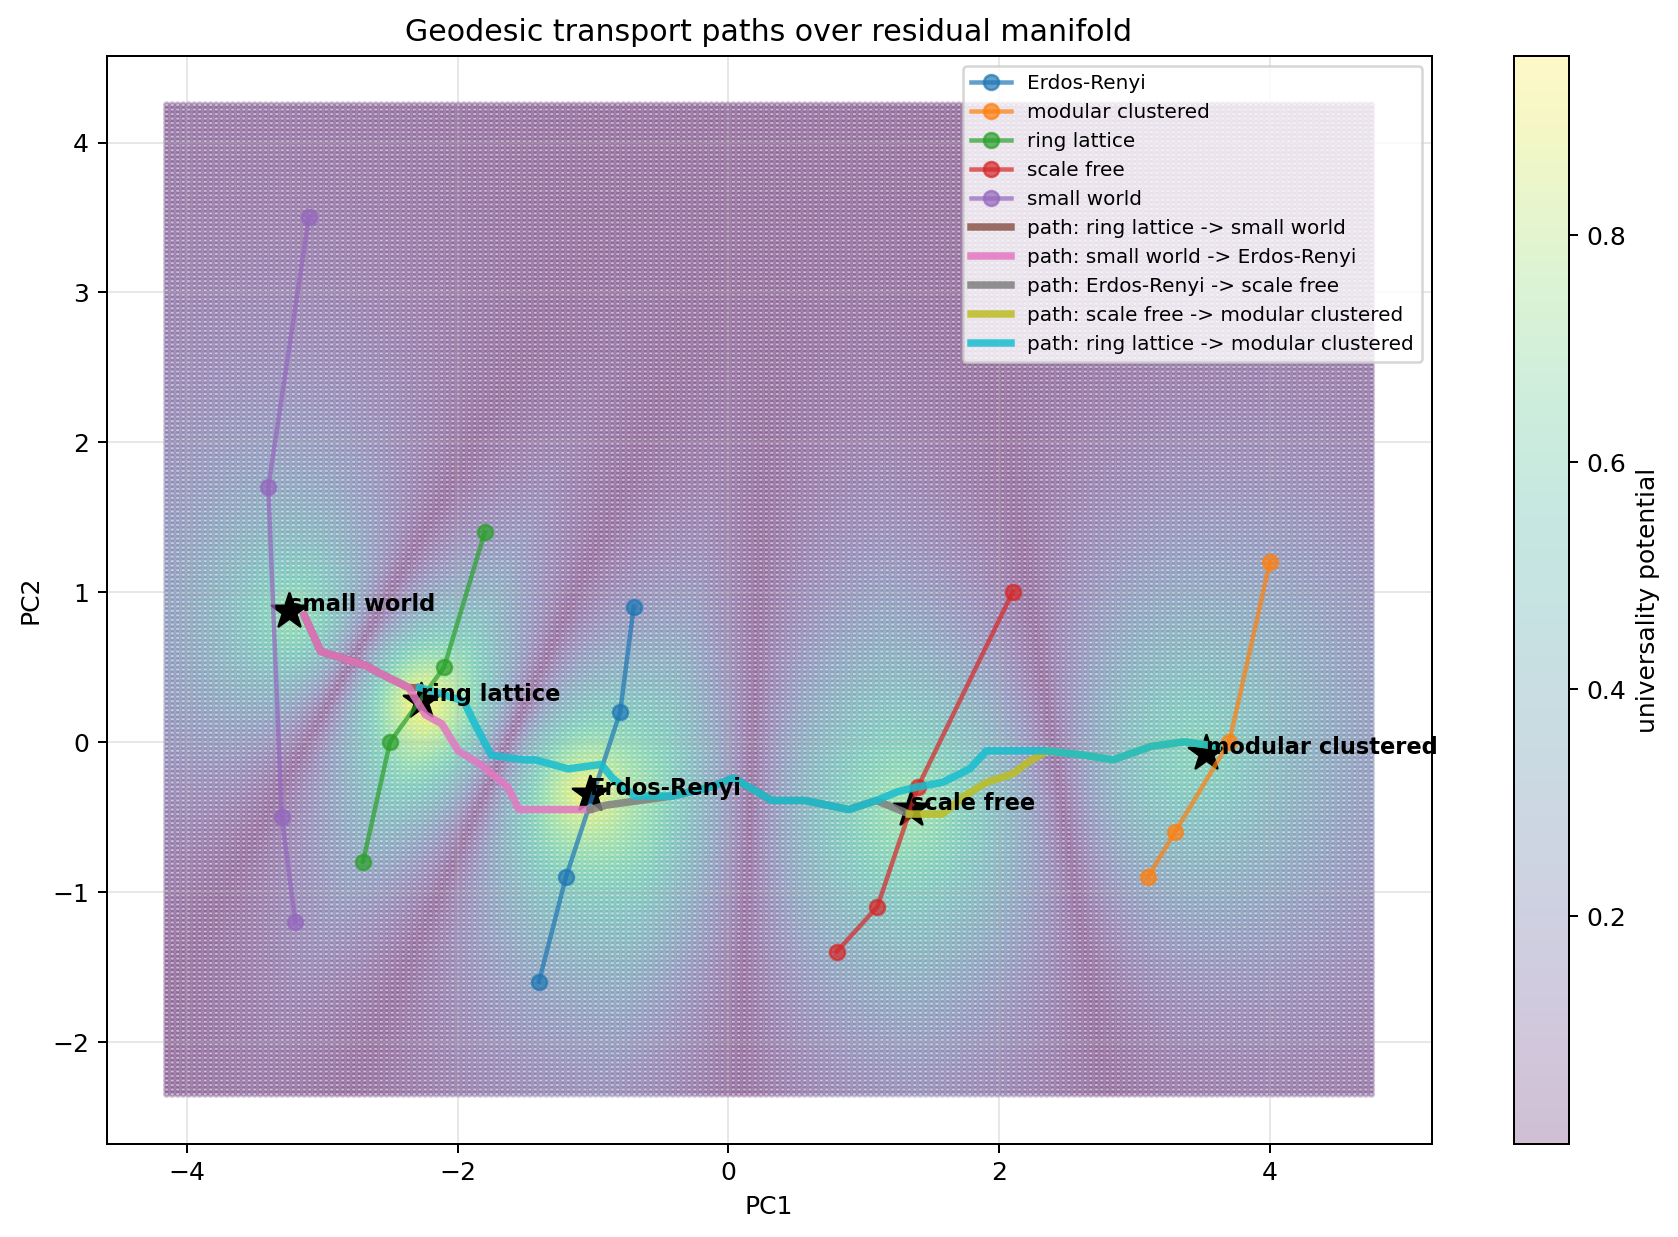
\includegraphics[width=0.82\textwidth]{figures/25_geodesic_transport_paths.png}
\caption{
Residual manifold geodesic transport structure. Transport continuity preserves topology-family adjacency relationships across residual manifold space.
}
\label{fig:transport_paths}
\end{figure}

Nearby topology families maintain shorter geodesic continuity distances while transport pathways preserve local manifold adjacency across scaling transitions.

\section{Bridgeability Structure}

Residual bridgeability operators quantify transport accessibility between topology families.

Bridgeability is represented:
\[
\mathcal{B}_{ij}
=
\exp(-d_g(i,j)).
\]

Figure~\ref{fig:bridgeability} shows bridgeability continuity structure.

\begin{figure}[H]
\centering
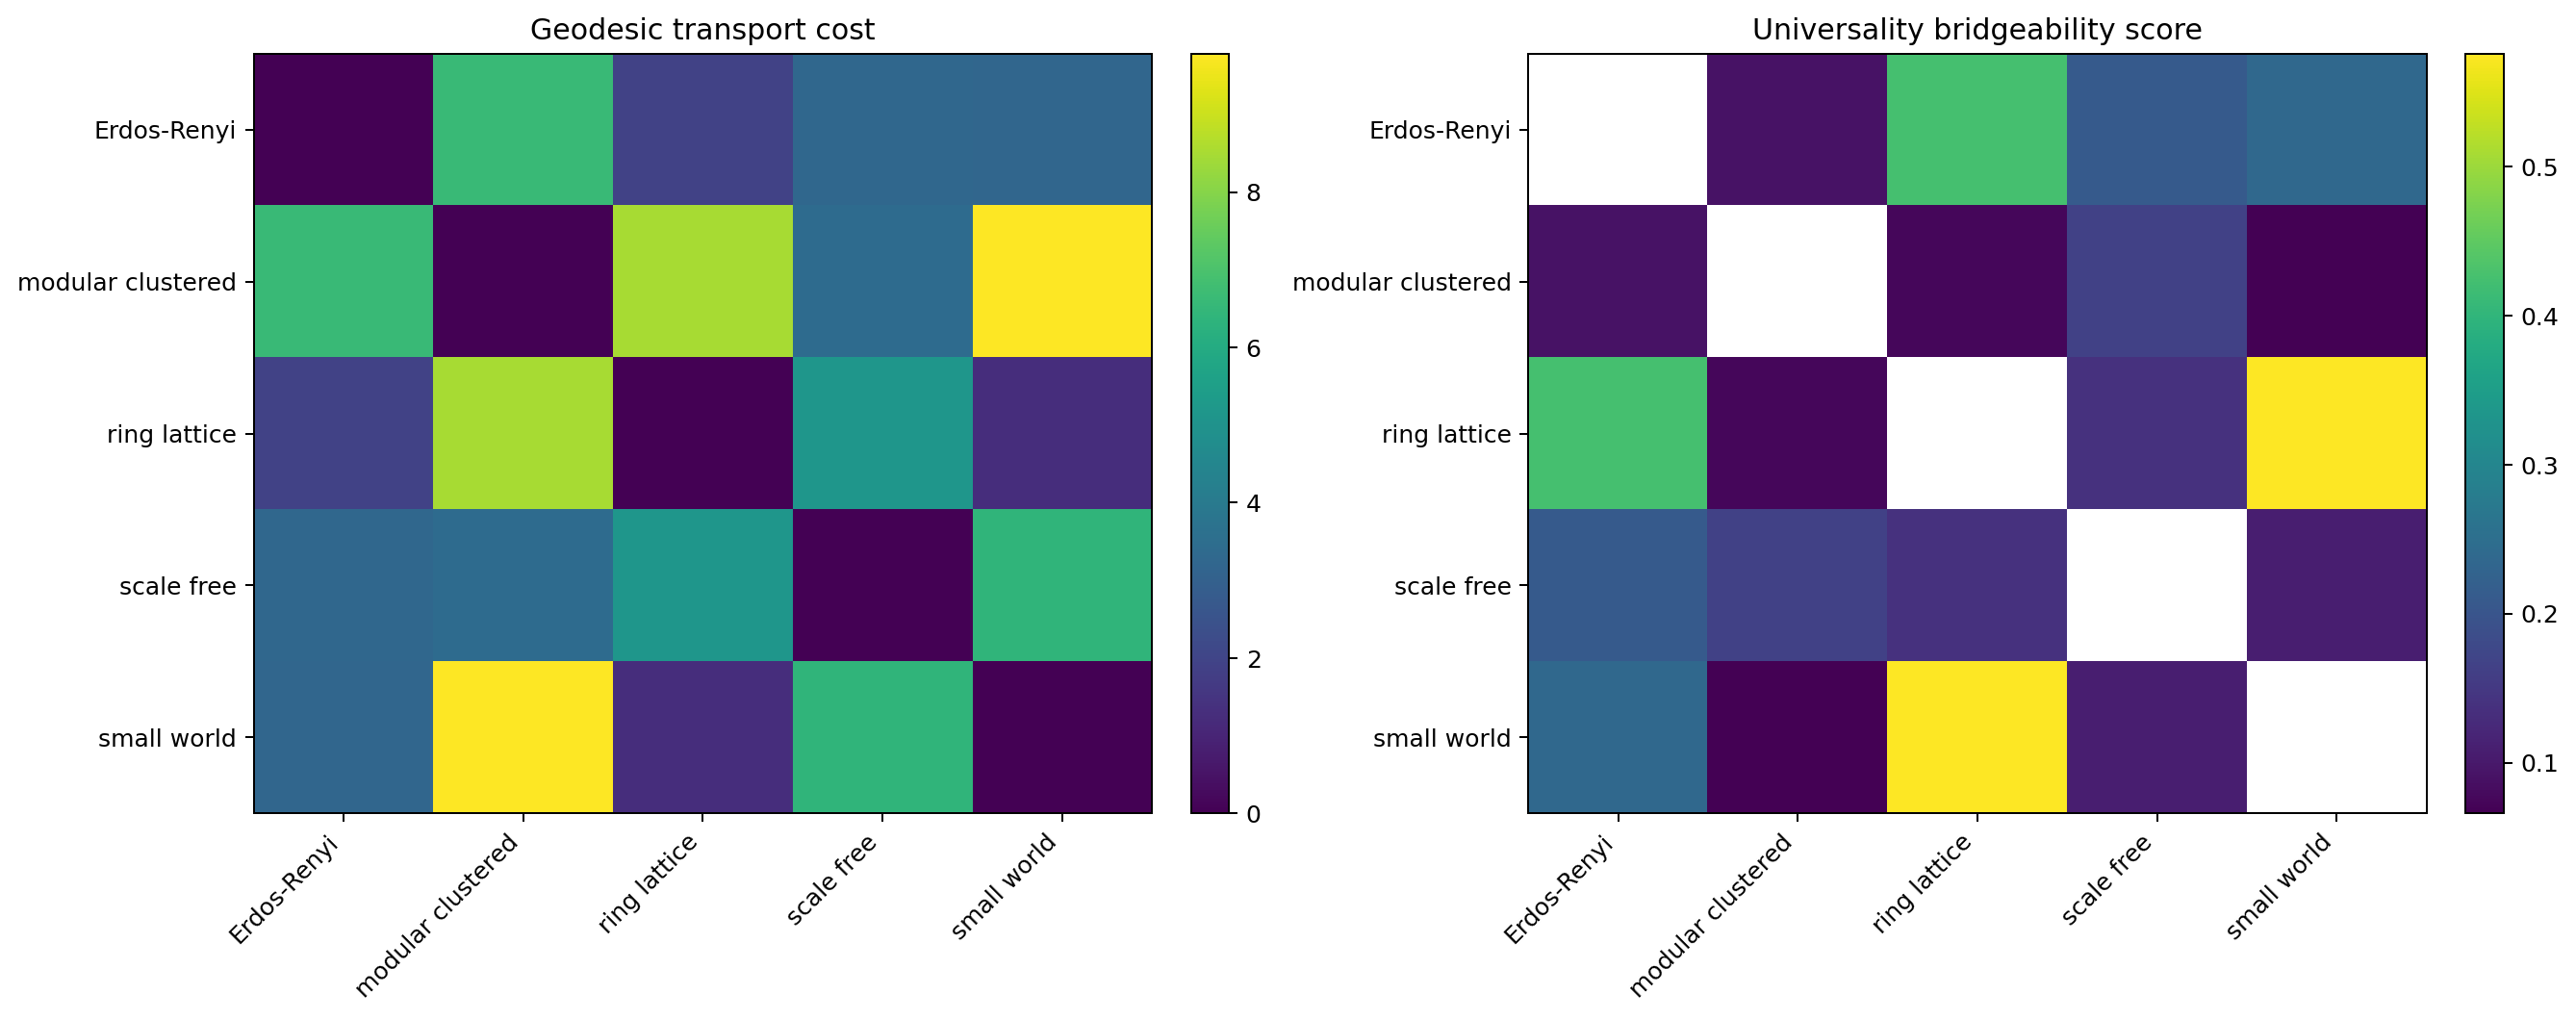
\includegraphics[width=0.72\textwidth]{figures/25_bridge_matrix_heatmap.png}
\caption{
Residual manifold bridgeability matrix. Bridgeability asymmetry reveals transport accessibility differences between topology families.
}
\label{fig:bridgeability}
\end{figure}

High bridgeability values indicate low residual transport resistance between topology families under geodesic manifold flow.

Small-world and ring-lattice systems exhibit strong mutual transport continuity, while modular-clustered and scale-free systems remain comparatively isolated under residual geodesic transport.

\section{Diffusion Persistence}

Diffusion persistence operators evaluate residual continuity under iterative propagation.

Diffusion evolution is defined:
\[
u_{t+1}
=
(I-\alpha L)u_t
\]
where \(L\) denotes the graph Laplacian.

Diffusion propagation operators are closely related to diffusion-map and Laplacian embedding constructions developed in spectral manifold learning \cite{coifman2006diffusion,belkin2003laplacian}.

Figure~\ref{fig:entropy_persistence} shows diffusion entropy growth and persistence decay.

\begin{figure}[H]
\centering
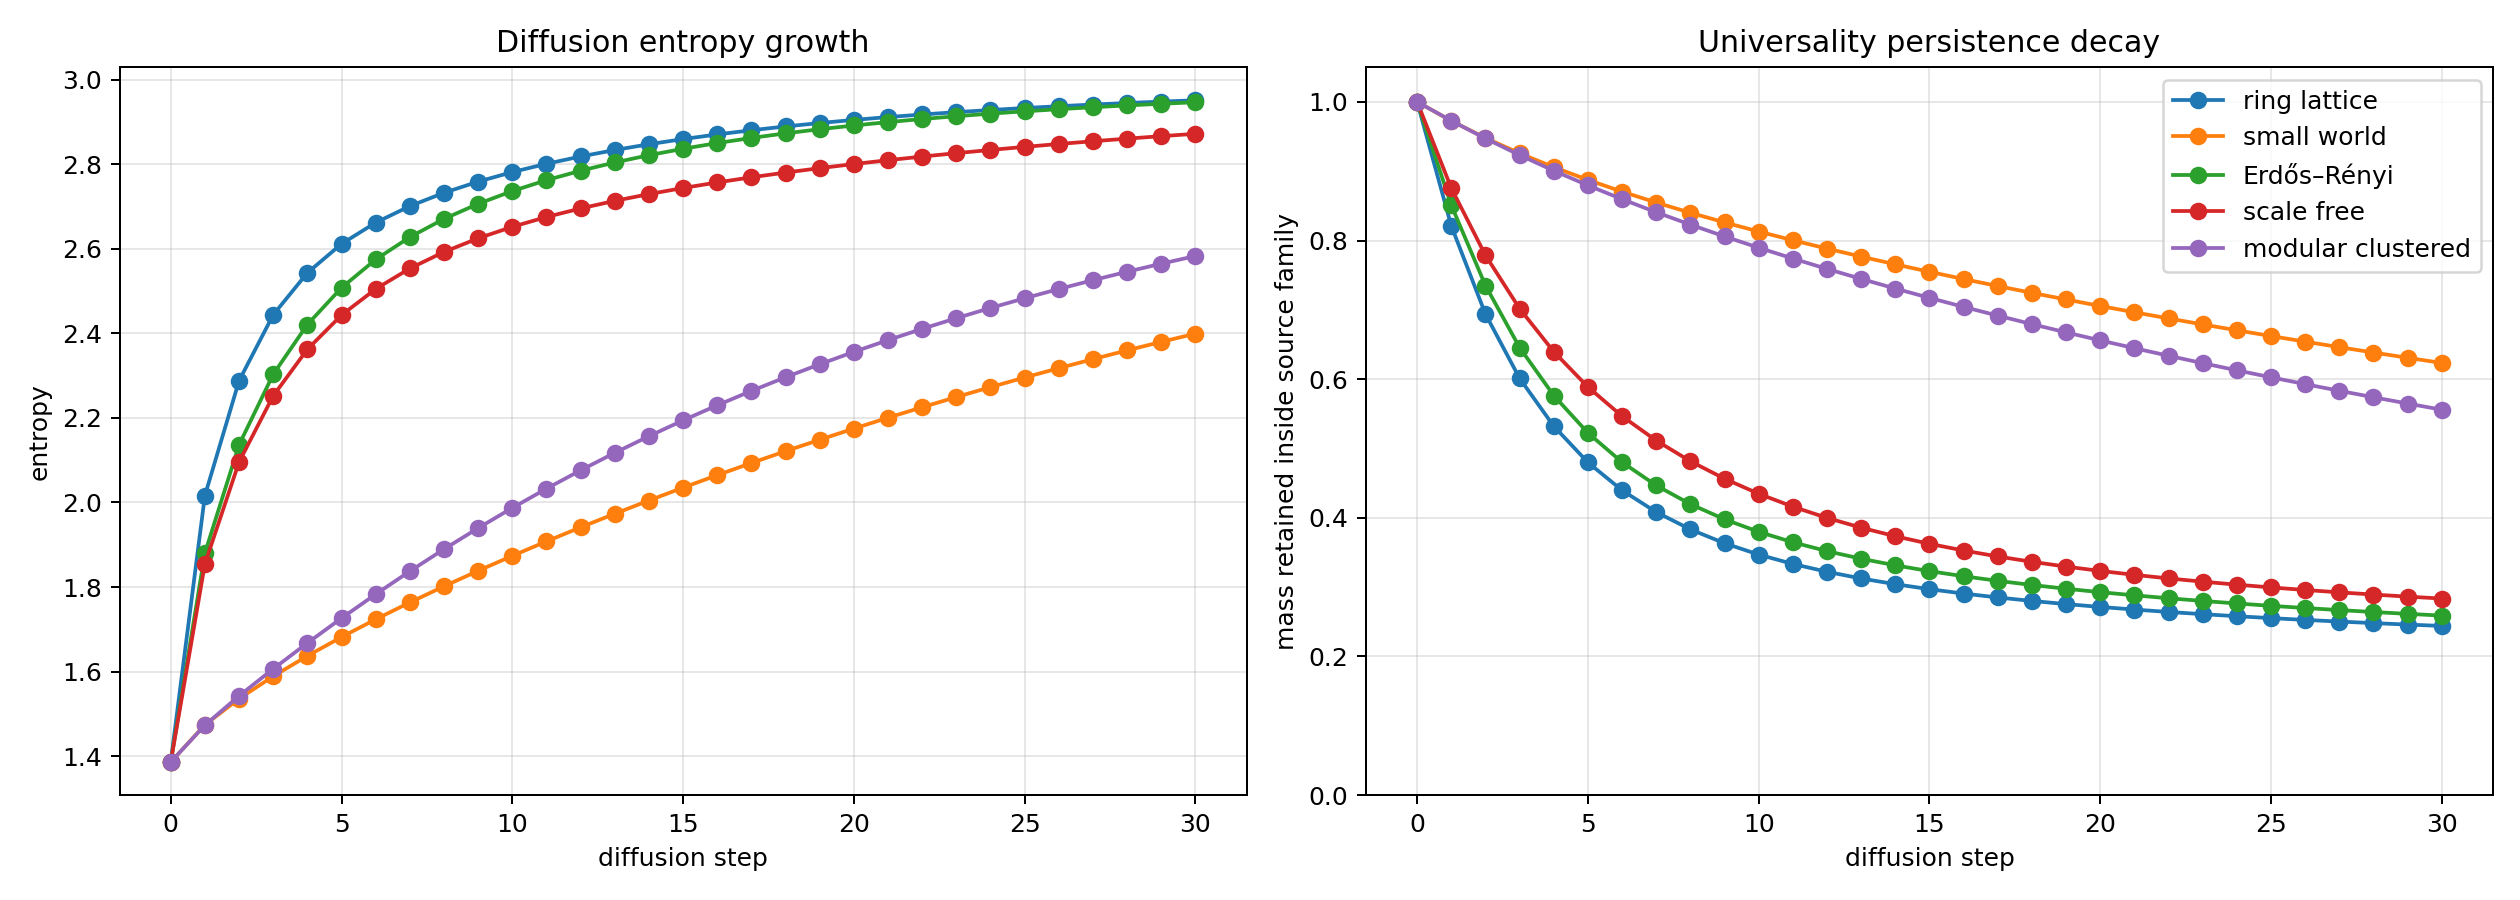
\includegraphics[width=\textwidth]{figures/26_entropy_and_persistence.png}
\caption{
Residual diffusion entropy growth and persistence decay across topology families. Diffusion-retained continuity remains family-consistent under iterative transport.
}
\label{fig:entropy_persistence}
\end{figure}

Diffusion propagation preserves topology-family neighborhood structure while local diffusion neighborhoods remain stable throughout iterative transport evolution.

\section{Residual Diffusion Geometry}

Residual diffusion neighborhoods are visualized through topology-family diffusion manifolds.

Figure~\ref{fig:diffusion_knn} shows diffusion neighborhood structure.

\begin{figure}[H]
\centering
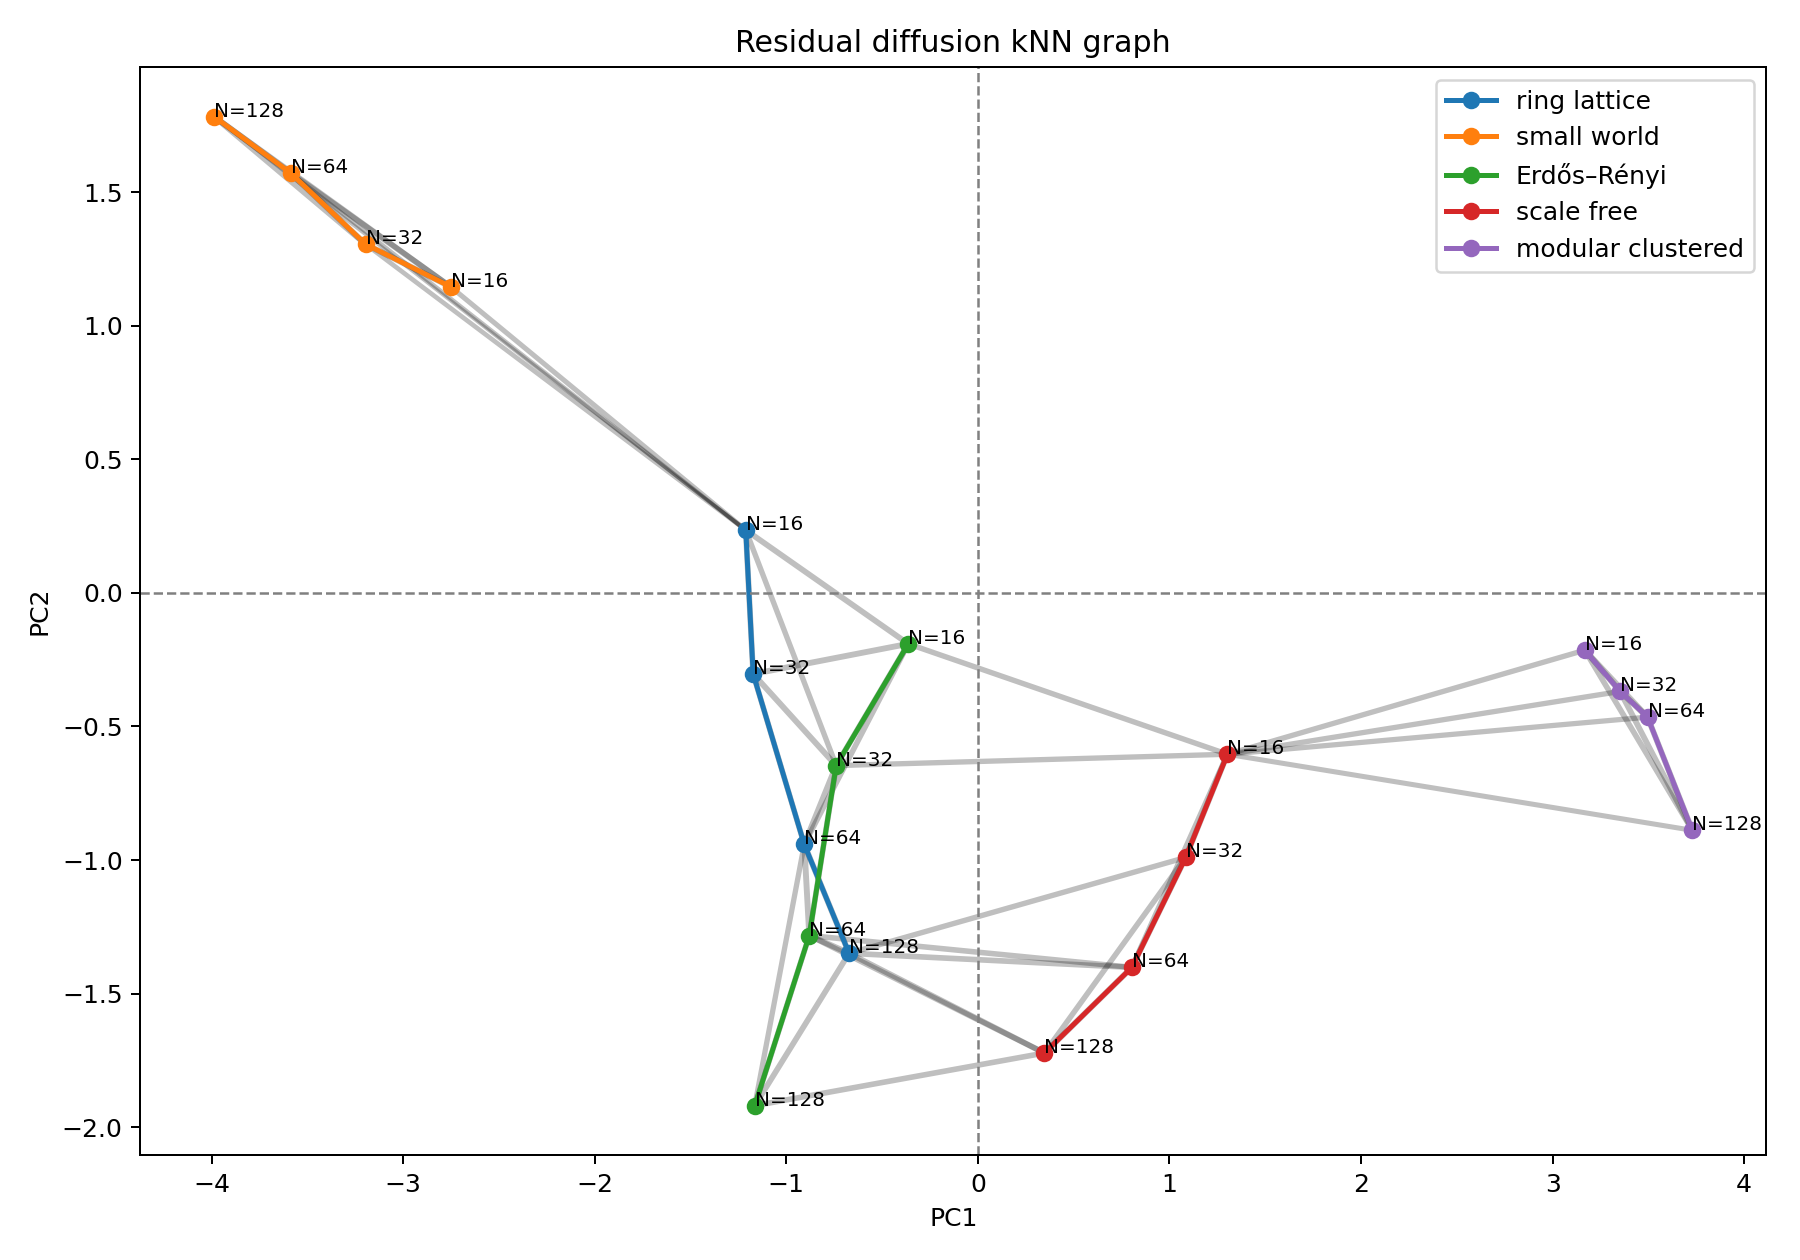
\includegraphics[width=0.82\textwidth]{figures/26_diffusion_knn_graph.png}
\caption{
Residual diffusion neighborhood graph. Diffusion continuity preserves family-local adjacency structure across graph scaling.
}
\label{fig:diffusion_knn}
\end{figure}

Diffusion continuity neighborhoods remain topology-localized while preserving manifold transport structure across residual operator evolution.

\section{Spectral Hierarchy Emergence}

Residual topology construction produces organized operator structure across topology families. Spectral embeddings, Laplacian eigensystems, and eigengap organization play central roles in spectral clustering and manifold representation methods \cite{ng2002spectral,chung1997spectral}. Rather than behaving as unstructured graph perturbations, residual manifolds generate cumulative spectral organization, transport-coupling transitions, and fragmentation hierarchies visible across Laplacian eigenspectra, spectral overlap structure, and cumulative operator accumulation.

\subsection{Topology-family spectral overlap}

Figure~\ref{fig:spectral_overlap_matrix} shows normalized spectral overlap between topology families.

\begin{figure}[H]
\centering
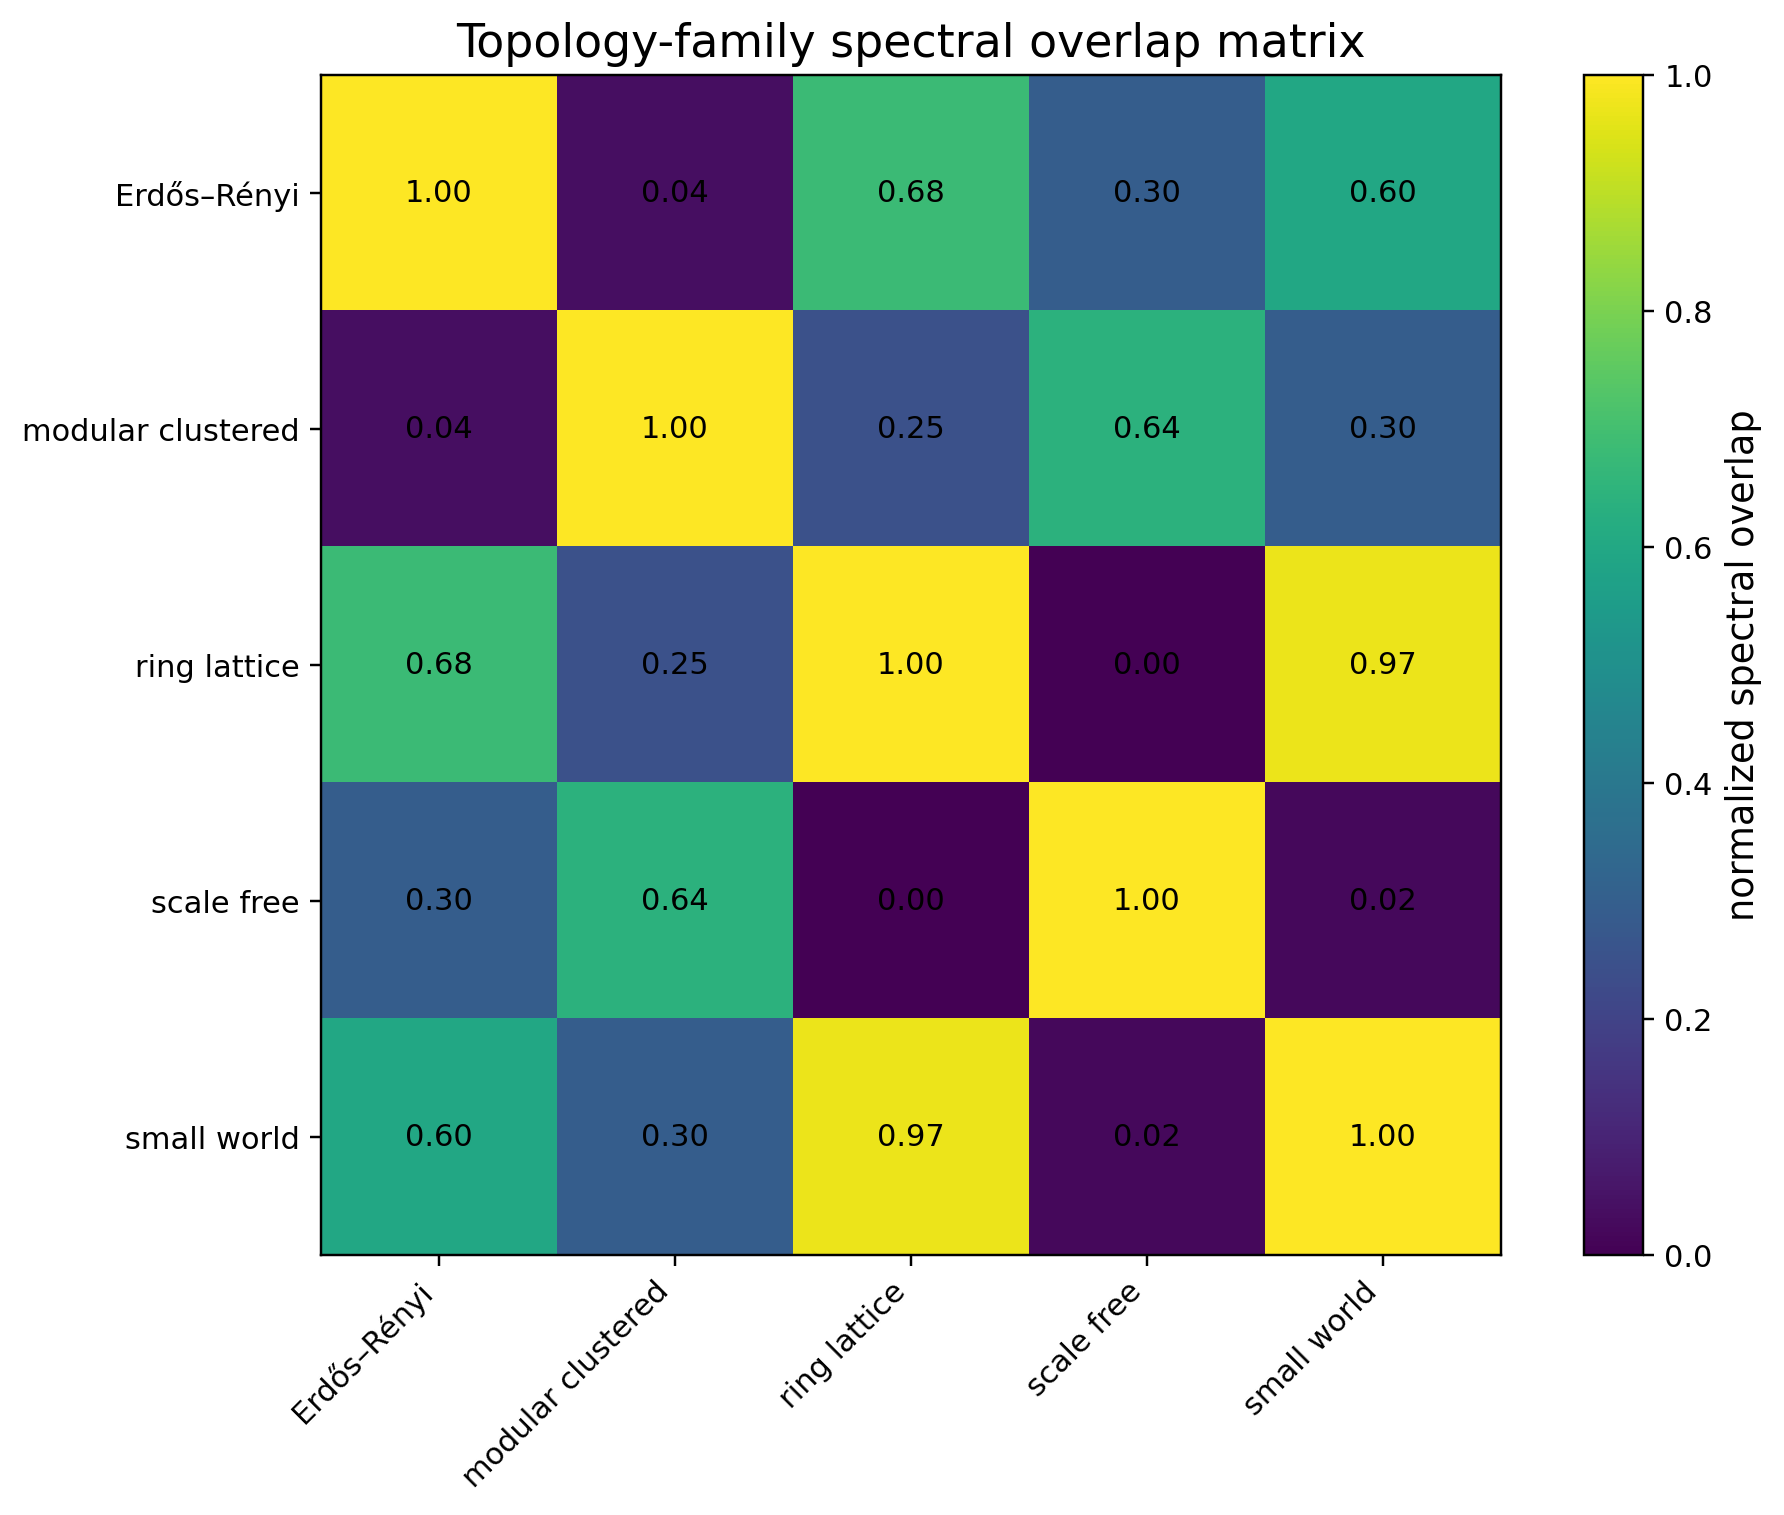
\includegraphics[width=0.88\textwidth]{figures/27_spectral_overlap_matrix.png}
\caption{
Normalized spectral overlap matrix across topology families. Ring-lattice and small-world systems maintain strong overlap structure, while modular-clustered and scale-free systems separate into distinct spectral transport regimes.
}
\label{fig:spectral_overlap_matrix}
\end{figure}

Spectral overlap reveals persistent transport compatibility across topology families. Ring-lattice and small-world systems exhibit high normalized overlap, indicating continuity-preserving transport structure across local neighborhoods and distributed coupling paths.

These overlap structures demonstrate that residual manifolds preserve measurable operator-family organization rather than collapsing into topology-independent spectral distributions.

\subsection{Topology-family spectral trajectories}

Figure~\ref{fig:spectral_trajectories} shows spectral trajectories across topology families and graph scales.

\begin{figure}[H]
\centering
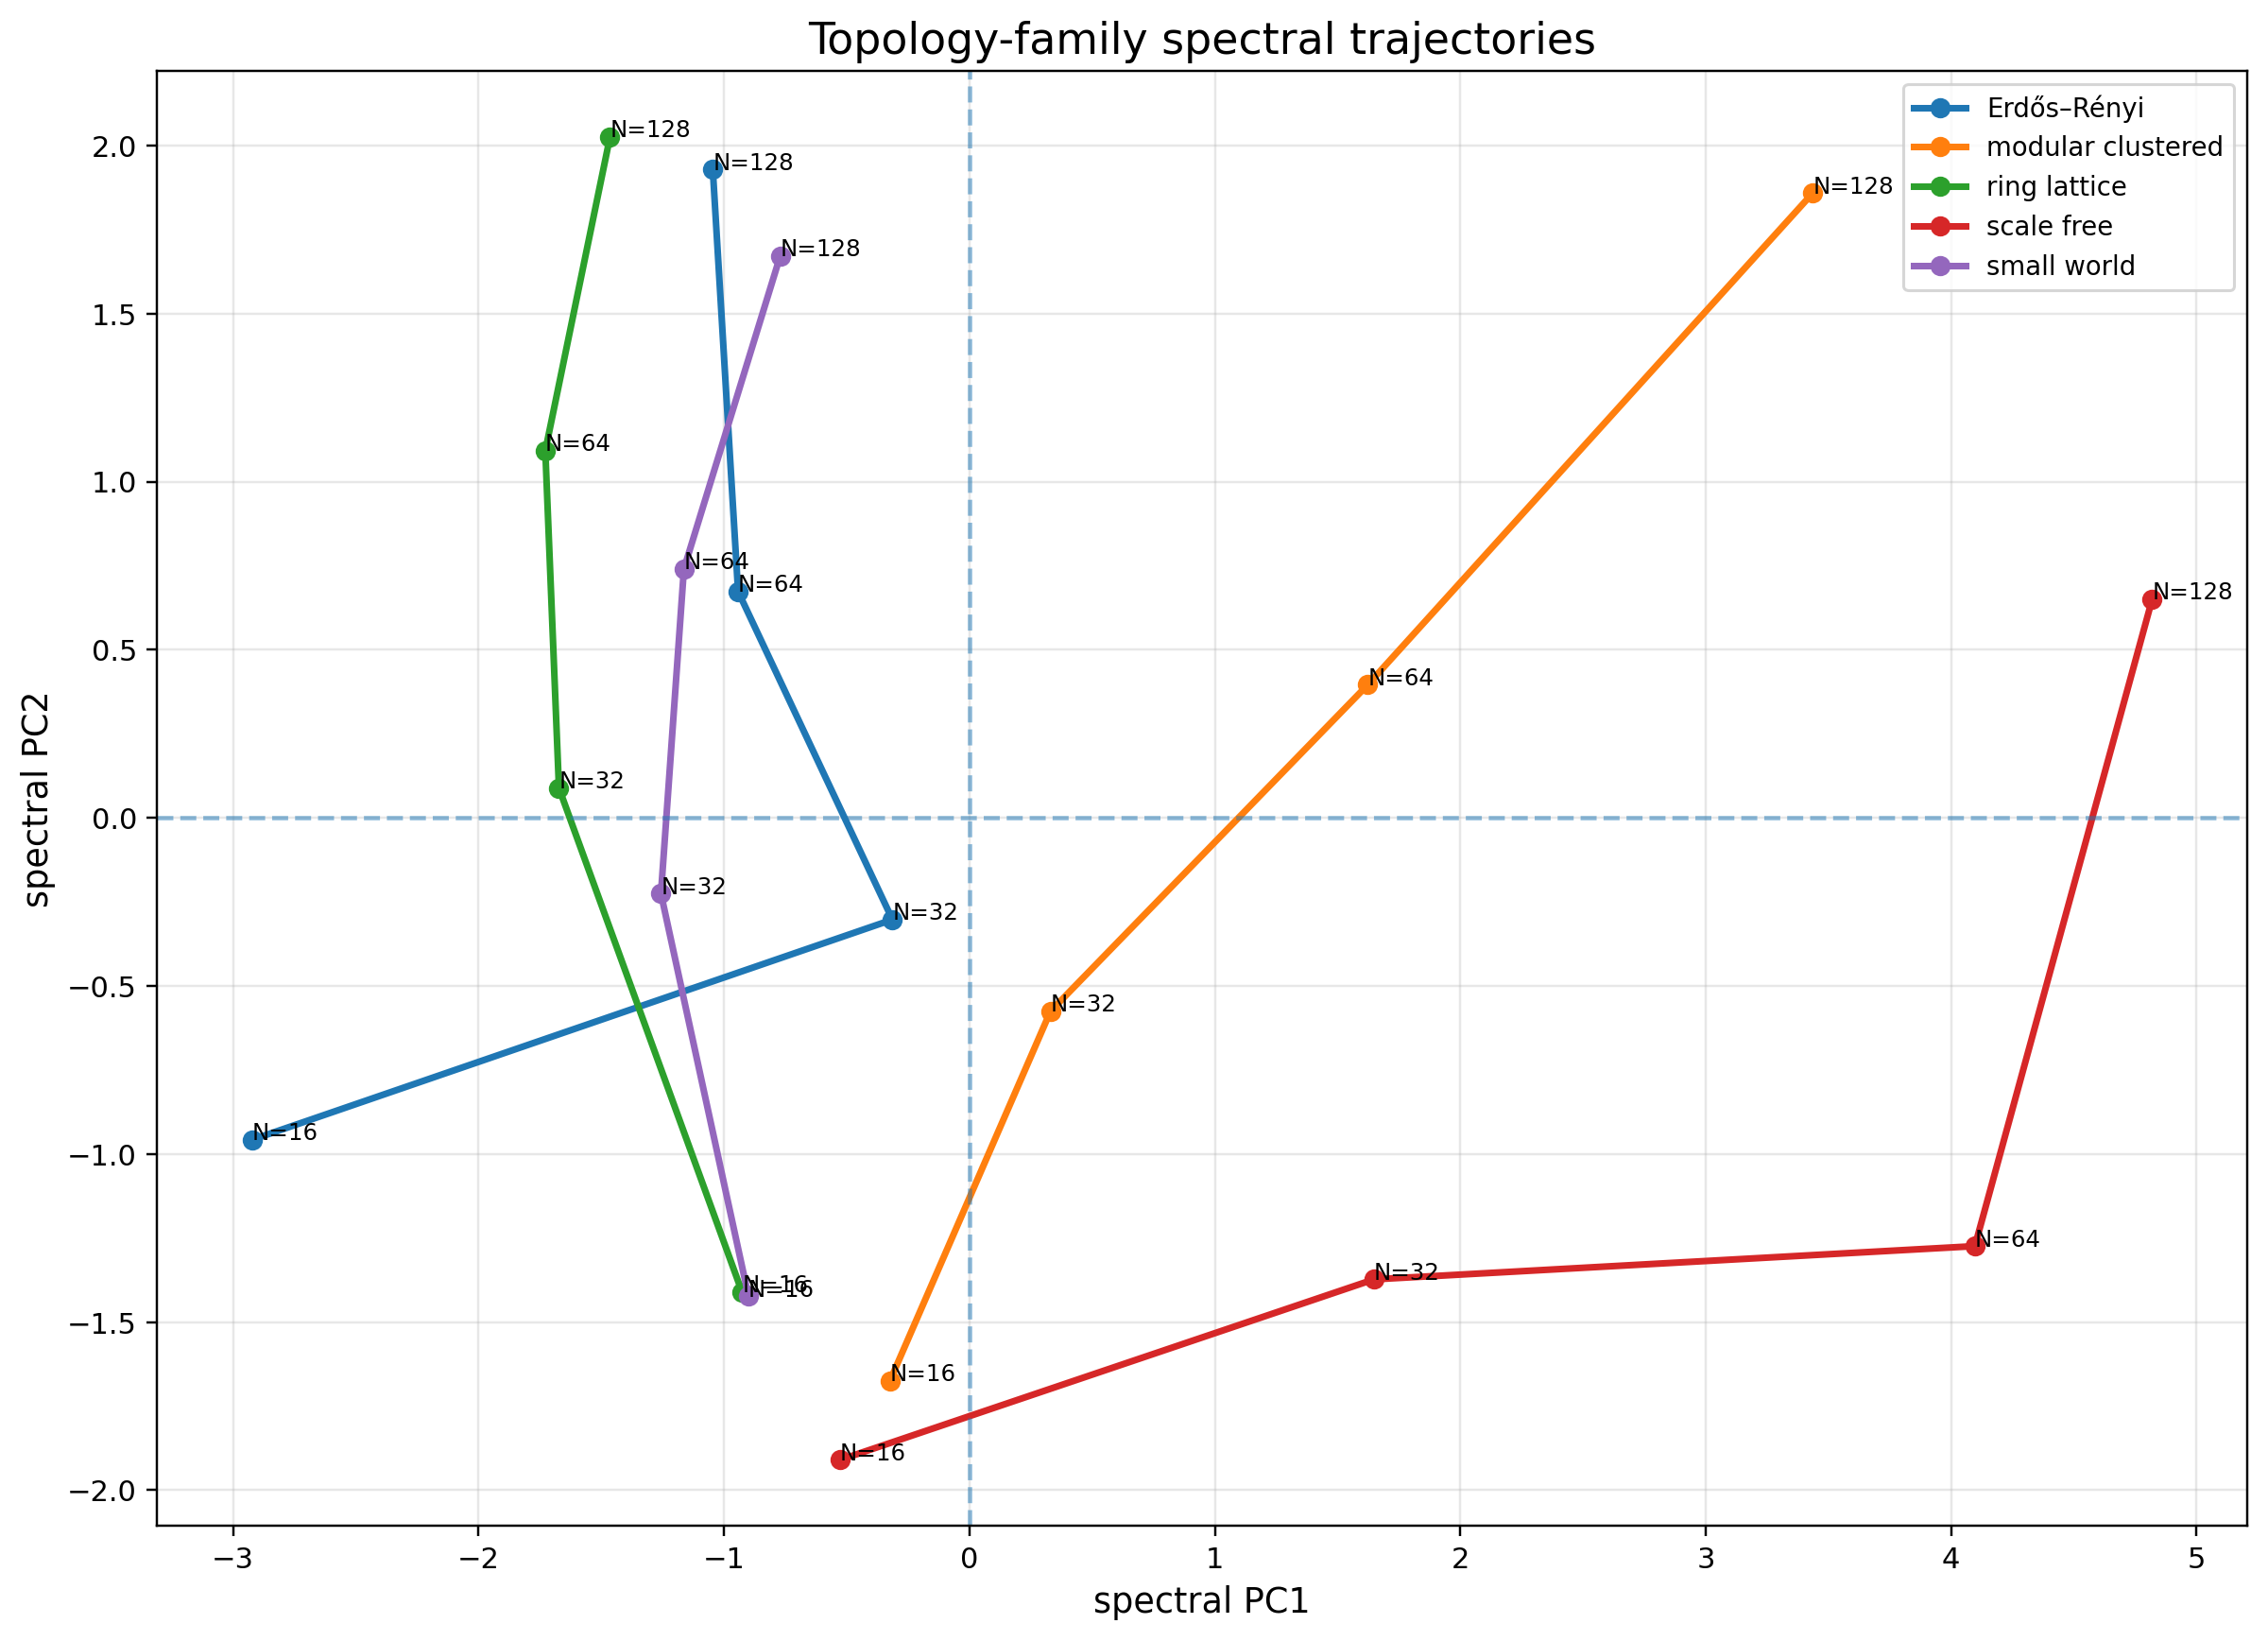
\includegraphics[width=0.92\textwidth]{figures/27_topology_family_spectral_trajectories.png}
\caption{
Topology-family spectral trajectories projected into principal spectral coordinates. Continuity-preserving systems remain clustered, while transport-dominant and fragmentation-dominant systems diverge across spectral phase space.
}
\label{fig:spectral_trajectories}
\end{figure}

Residual spectral trajectories organize into coherent topology-family paths across increasing graph scales.

Ring-lattice and small-world systems remain localized within continuity-preserving spectral regions, while modular-clustered systems evolve through intermediate transport-coupling regions. Scale-free systems diverge into fragmentation-dominant spectral regions associated with hub concentration and heterogeneous transport pathways.

\subsection{Residual spectral accumulation}

Residual operator organization becomes increasingly visible through cumulative spectral accumulation.

Define cumulative spectral mass:
\[
M(k)=
\frac{
\sum_{i=0}^{k}\lambda_i
}{
\sum_{i=0}^{n}\lambda_i
}
\]

where \(\lambda_i\) denotes ordered residual Laplacian eigenvalues.

Figure~\ref{fig:spectral_entropy_curve} shows cumulative spectral entropy accumulation.

\begin{figure}[H]
\centering
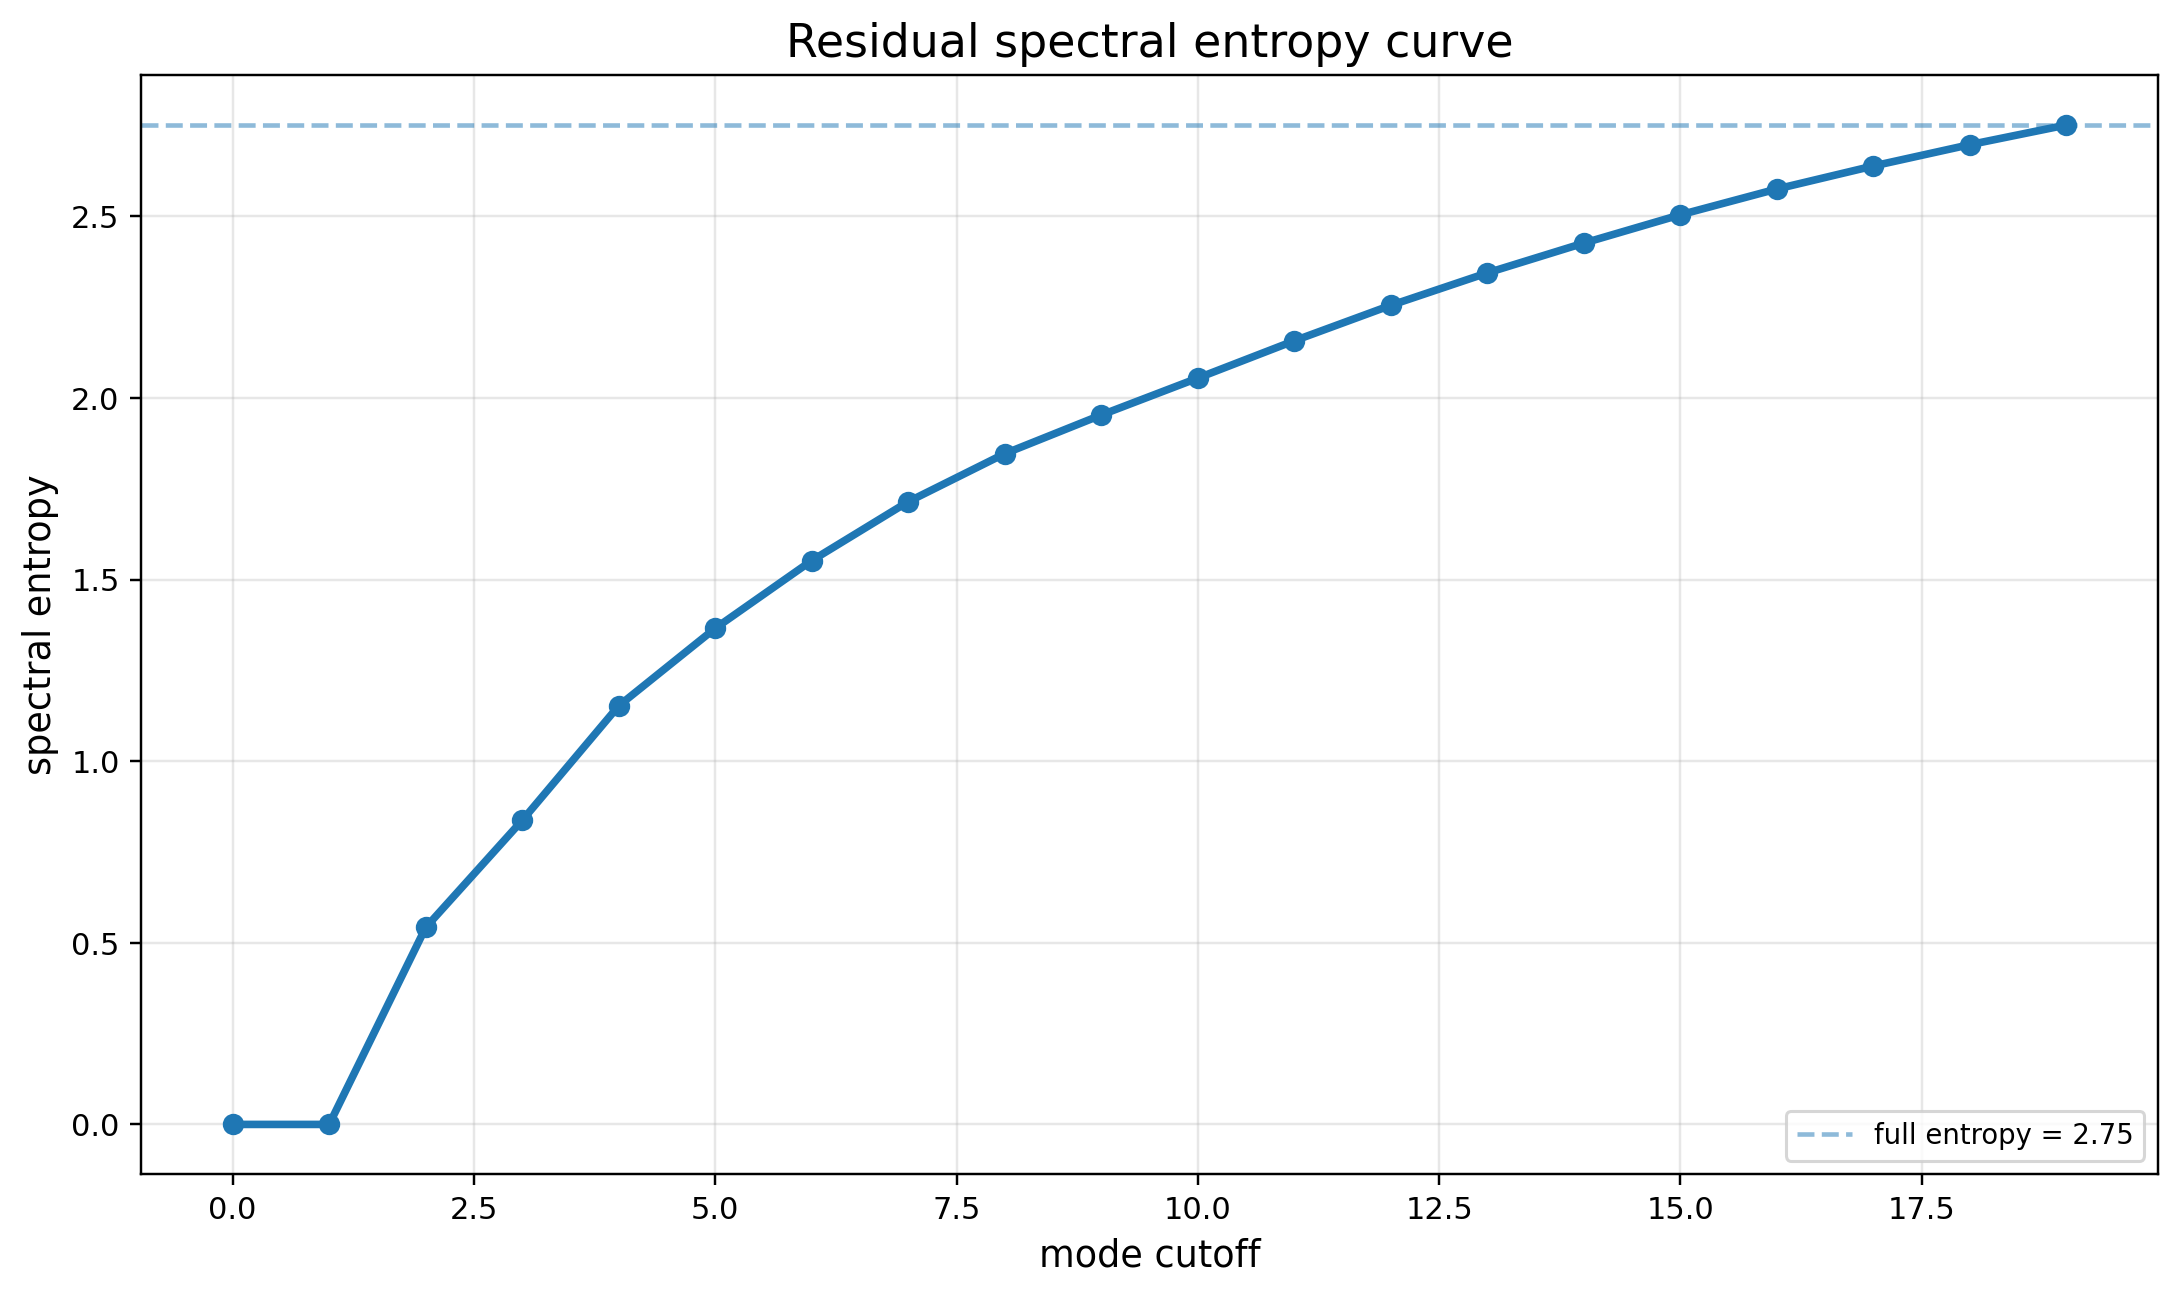
\includegraphics[width=0.78\textwidth]{figures/27_spectral_entropy_curve.png}
\caption{
Residual spectral entropy accumulation across increasing mode cutoff. Spectral organization grows progressively through cumulative operator inclusion.
}
\label{fig:spectral_entropy_curve}
\end{figure}

Entropy accumulation grows smoothly across increasing mode inclusion, indicating progressively structured operator participation rather than abrupt random spectral saturation.

Figure~\ref{fig:cumulative_residual_spectrum} shows cumulative residual spectral mass organization.

\begin{figure}[H]
\centering
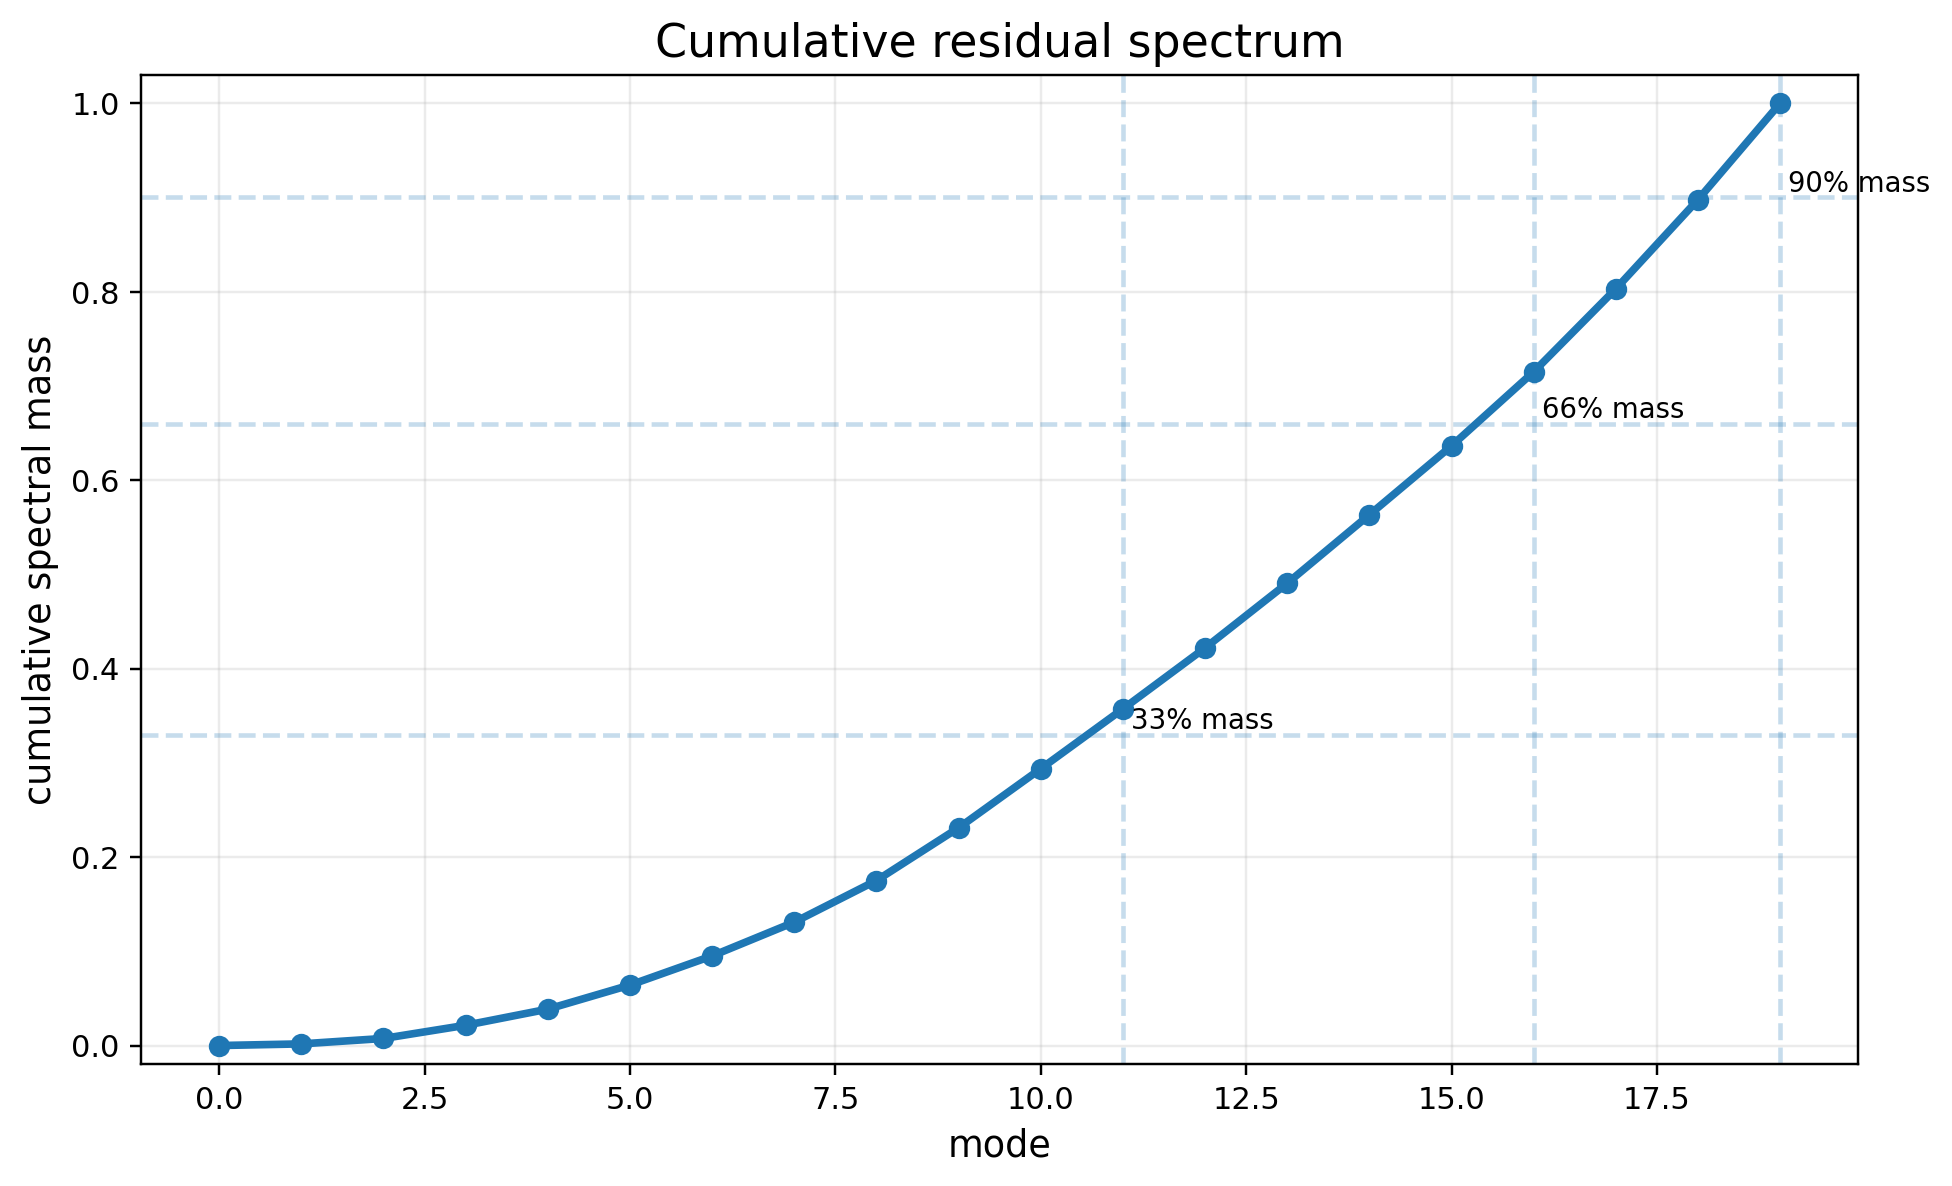
\includegraphics[width=0.88\textwidth]{figures/27_cumulative_residual_spectrum.png}
\caption{
Cumulative residual spectral mass across ordered operator modes. Distinct accumulation thresholds emerge across continuity, transport, and fragmentation-dominant operator regions.
}
\label{fig:cumulative_residual_spectrum}
\end{figure}

Cumulative spectral mass exhibits organized threshold structure across operator bands. Lower-frequency modes contribute continuity-preserving structure, intermediate modes contribute transport-coupling organization, and higher-frequency modes contribute fragmentation dynamics and localized spectral separation.

\subsection{Eigengap hierarchy and regime transitions}

Residual eigengap structure reveals organized regime transitions across operator hierarchy levels.

Define residual eigengap spacing:
\[
\Delta_k=\lambda_{k+1}-\lambda_k
\]

where \(\lambda_k\) denotes ordered Laplacian eigenvalues.

Figure~\ref{fig:cumulative_eigengap_hierarchy} shows cumulative eigengap hierarchy organization.

\begin{figure}[H]
\centering
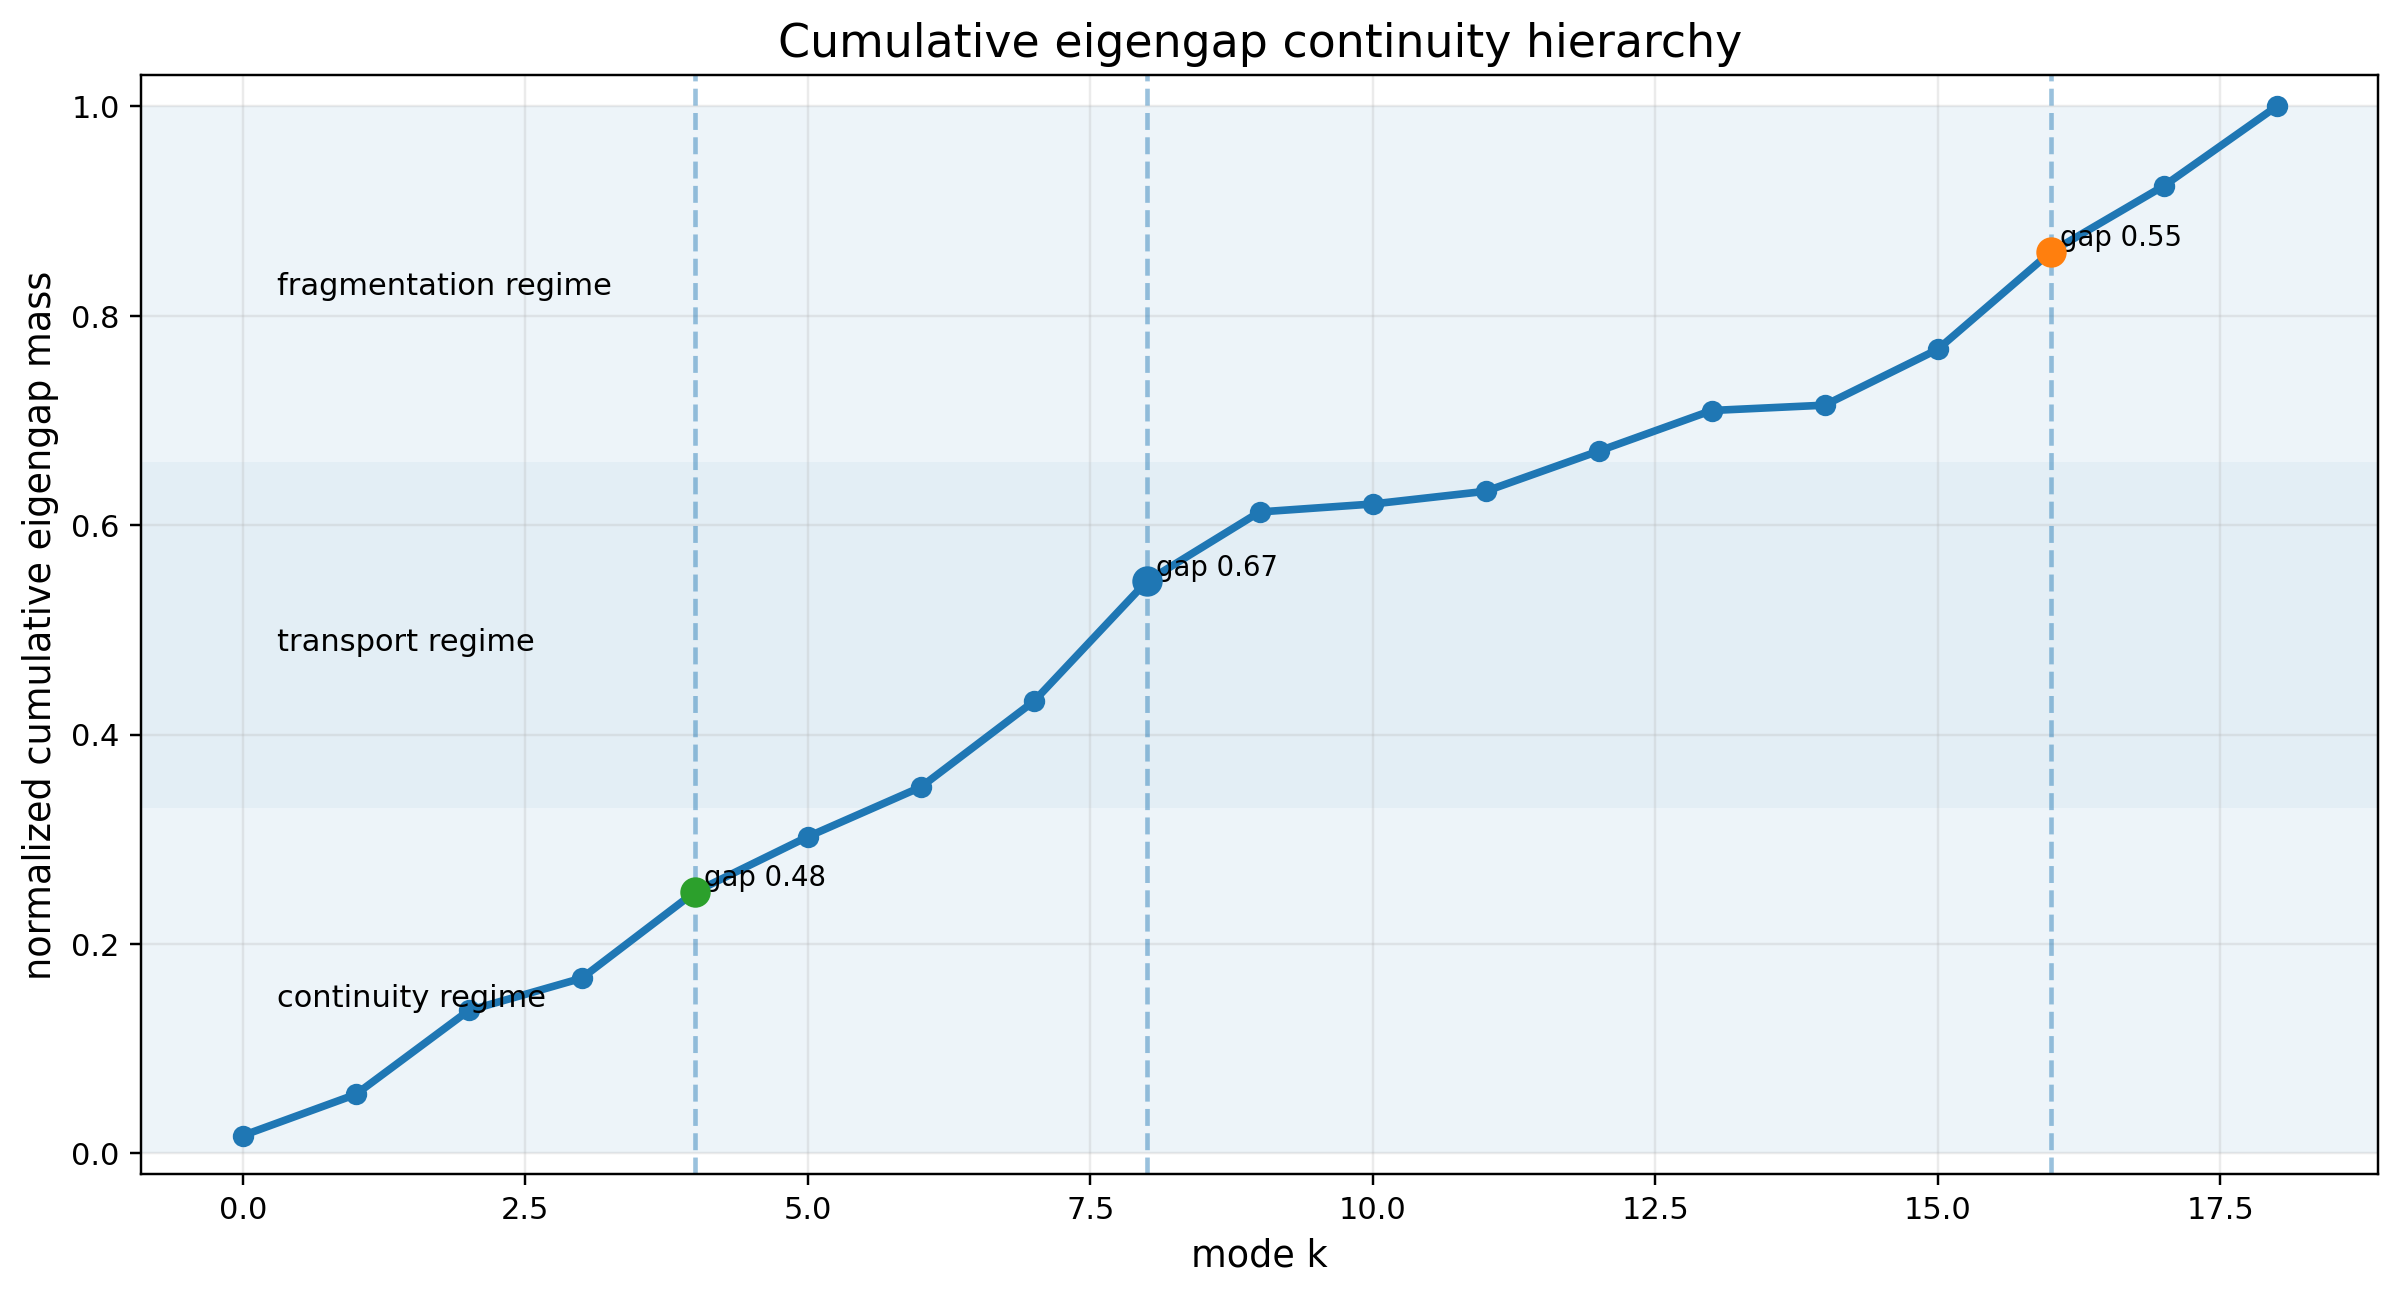
\includegraphics[width=0.92\textwidth]{figures/27_cumulative_eigengap_hierarchy.png}
\caption{
Cumulative eigengap hierarchy across ordered operator modes. Distinct continuity, transport-coupling, and fragmentation regimes emerge through cumulative eigengap organization.
}
\label{fig:cumulative_eigengap_hierarchy}
\end{figure}

The cumulative eigengap hierarchy separates into three operator regimes:

\begin{itemize}
\item continuity regime,
\item transport-coupling regime,
\item fragmentation regime.
\end{itemize}

Low-frequency continuity modes preserve global manifold organization and stable transport coherence. Intermediate transport-coupling modes organize cross-manifold interaction structure and bridge dynamics. Higher-frequency fragmentation modes isolate localized transport separation and residual operator concentration.

Figure~\ref{fig:residual_laplacian_eigenspectrum} shows the full residual Laplacian eigenspectrum with regime transitions annotated directly on the spectrum.

\begin{figure}[H]
\centering
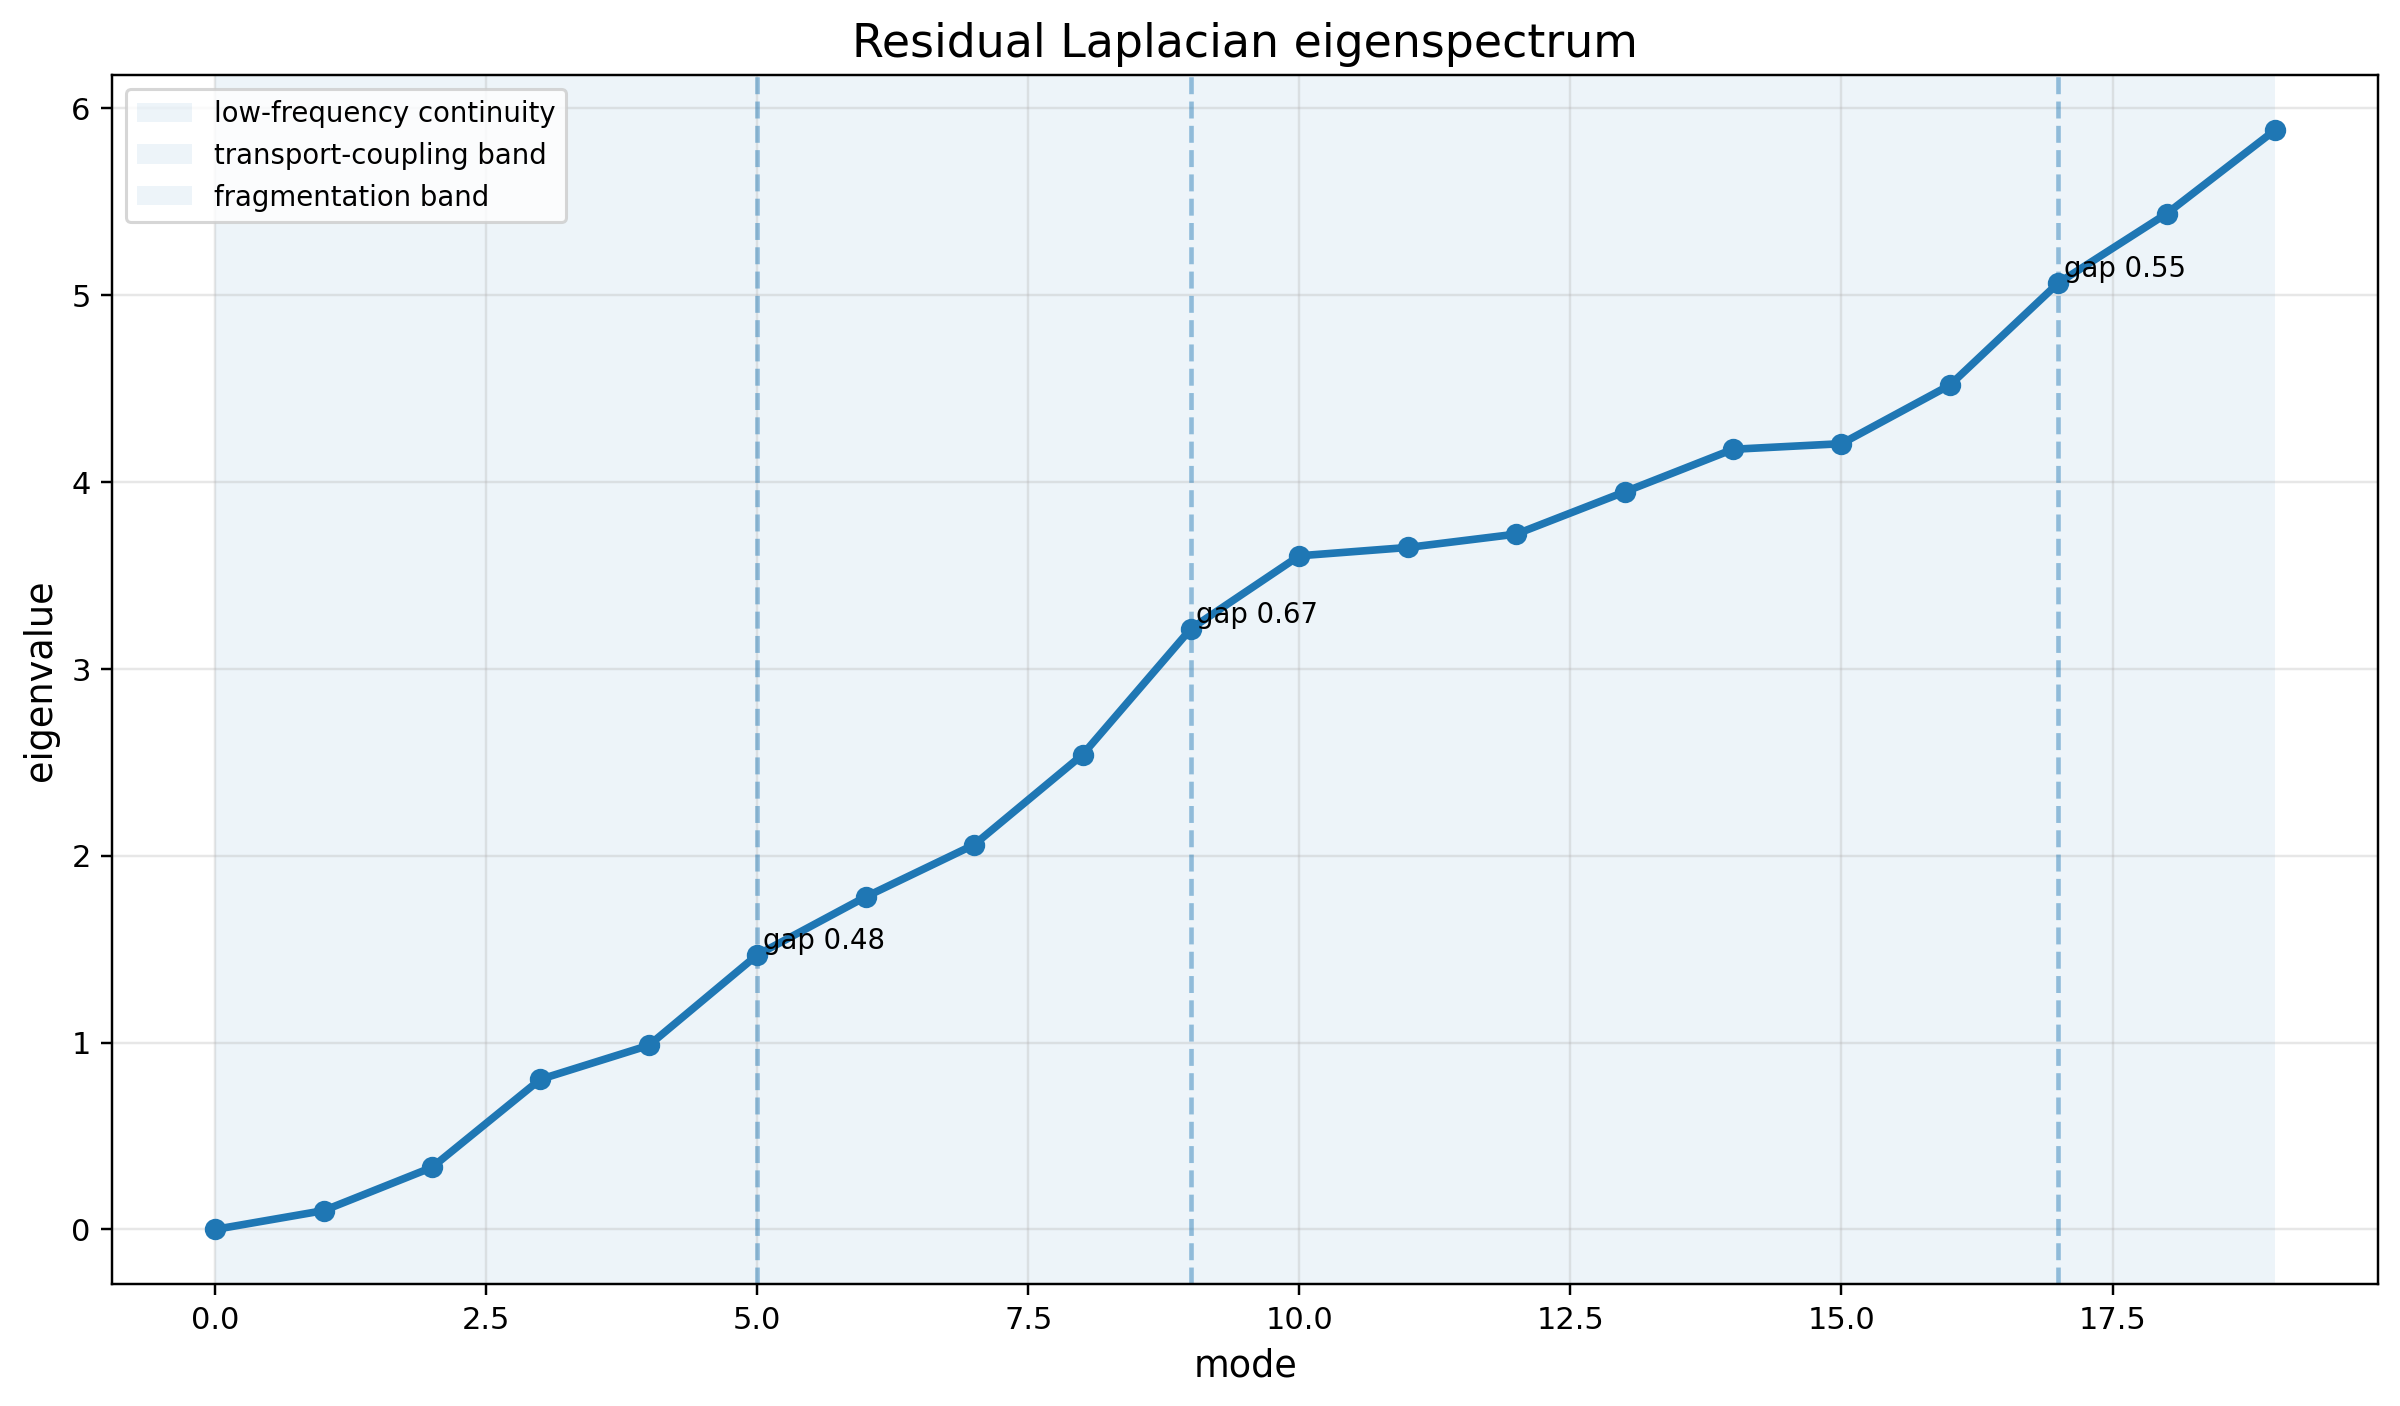
\includegraphics[width=0.92\textwidth]{figures/27_residual_laplacian_eigenspectrum.png}
\caption{
Residual Laplacian eigenspectrum with continuity, transport-coupling, and fragmentation hierarchy regions. Dominant eigengap transitions separate organized operator regimes across the residual manifold.
}
\label{fig:residual_laplacian_eigenspectrum}
\end{figure}

Low-order spectral bands preserve global continuity structure, while higher-order bands progressively localize topology-family fragmentation and transport resistance.

\subsection{Spectral hierarchy decomposition}

Figure~\ref{fig:spectral_hierarchy_decomposition} summarizes cumulative spectral hierarchy decomposition across operator bands.

\begin{figure}[H]
\centering
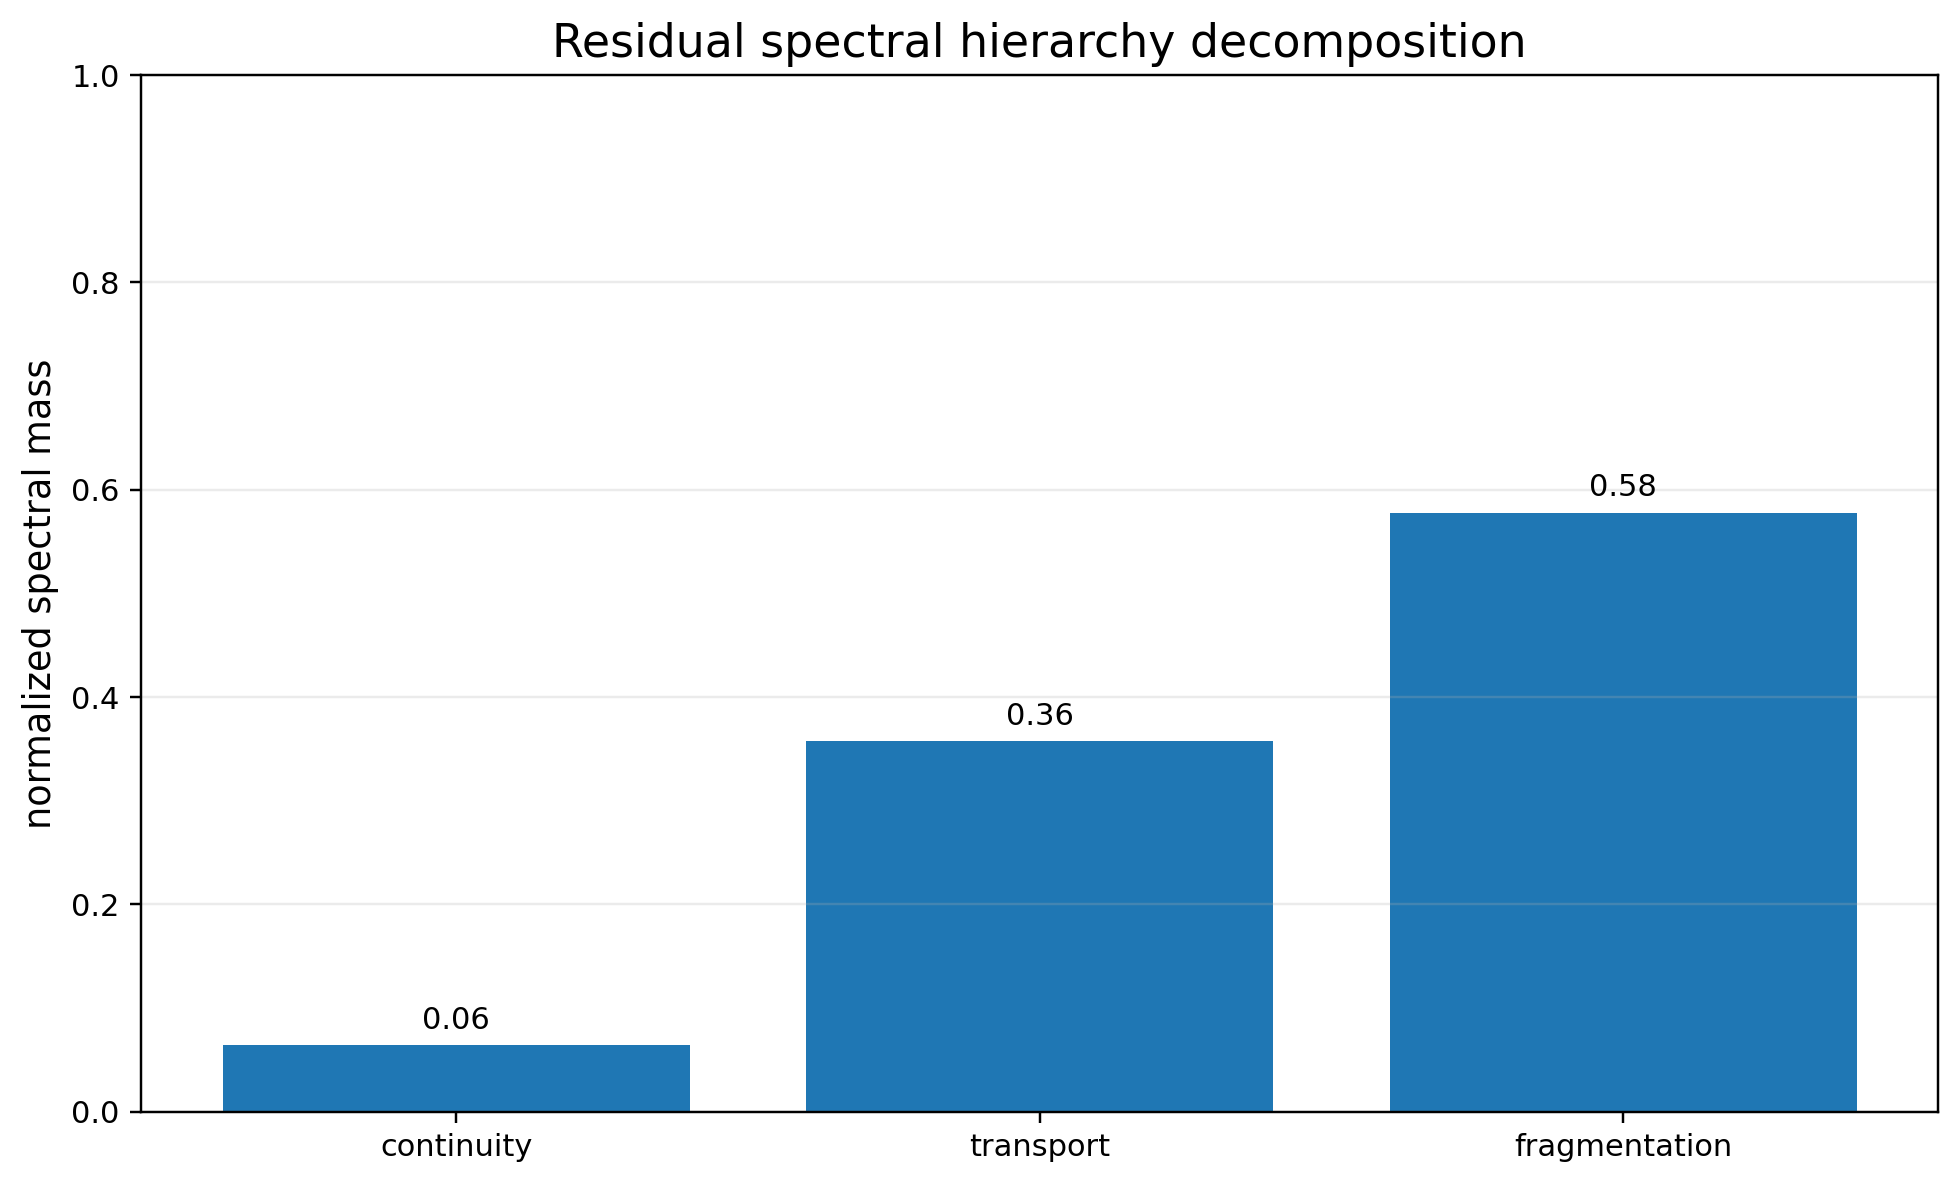
\includegraphics[width=0.72\textwidth]{figures/27_spectral_hierarchy_decomposition.png}
\caption{
Residual spectral hierarchy decomposition across continuity, transport, and fragmentation operator bands.
}
\label{fig:spectral_hierarchy_decomposition}
\end{figure}

Spectral decomposition compresses residual operator organization into three dominant hierarchy regions. Continuity modes contribute stable manifold coherence, transport modes contribute bridge alignment and distributed coupling, and fragmentation modes contribute localized residual concentration.

This decomposition demonstrates that residual manifolds preserve structured operator organization across topology families, transport pathways, and spectral hierarchy transitions simultaneously.

\section{Results Summary}

\begin{table}[H]
\centering
\caption{Residual operator hierarchy summary across topology families.}
\begin{tabular}{lll}
\toprule
Measurement & Dominant Structure & Operator Role \\
\midrule
Density geometry & topology-localized support & continuity reconstruction \\
Geodesic transport & adjacency preservation & transport coupling \\
Diffusion persistence & neighborhood retention & propagation continuity \\
Spectral overlap & topology-family alignment & operator compatibility \\
Eigengap hierarchy & regime partitioning & hierarchy emergence \\
\bottomrule
\end{tabular}
\end{table}

\section{Operator Hierarchy}

Residual manifold operators form a coupled continuity hierarchy spanning density geometry, transport continuity, diffusion persistence, and spectral decomposition. This coupled hierarchy combines spectral graph structure, diffusion geometry, and manifold transport organization within a unified residual operator framework \cite{chung1997spectral,coifman2006diffusion,villani2008optimal}.

Density operators reconstruct topology-localized support regions.

Transport operators preserve manifold adjacency across geodesic transport pathways.

Diffusion operators preserve family-consistent neighborhood organization under iterative propagation.

Spectral operators partition local continuity regimes from large-scale topology-family transition structure.

The resulting hierarchy produces a multi-scale residual operator framework linking:

\begin{itemize}
\item local manifold density,
\item transport accessibility,
\item diffusion persistence,
\item spectral continuity structure.
\end{itemize}

Residual operator composition may therefore be represented:
\[
\mathcal{O}_{\mathrm{residual}}
=
\mathcal{S}
\circ
\mathcal{D}
\circ
\mathcal{T}
\circ
\rho
\]

where:
\[
\rho
\rightarrow
\mathcal{T}
\rightarrow
\mathcal{D}
\rightarrow
\mathcal{S}
\]

correspond respectively to density reconstruction, transport continuity, diffusion propagation, and spectral decomposition.

Across all measured operators, residual manifold organization remains stable while resisting residual collapse and spectral mixing under graph scaling transitions.

\section{Extensions and Future Directions}

The residual operator hierarchy developed here naturally extends toward broader classes of transport, diffusion, and spectral manifold systems.

Current experiments evaluate synthetic topology families across controlled graph scaling regimes. Similar operator constructions may be extended across:

\begin{itemize}
\item weighted transport manifolds,
\item temporal graph evolution,
\item adaptive diffusion systems,
\item multi-layer topology operators,
\item learned embedding geometries,
\item stochastic transport environments.
\end{itemize}

Several additional operator directions emerge directly from the present hierarchy construction:

\begin{itemize}
\item operator composition dynamics,
\item spectral transport flow,
\item multi-scale diffusion operators,
\item continuity-energy minimization,
\item topology phase transitions,
\item spectral persistence landscapes.
\end{itemize}

Residual eigengap hierarchy measurements suggest that continuity, transport, and fragmentation regimes remain measurable across substantially larger graph systems and higher-dimensional manifold embeddings.

Future operator constructions may therefore extend residual manifold analysis toward broader classes of geometric transport systems, spectral continuity models, and multi-scale topology evolution frameworks.

\section{Conclusion}

Residual manifold operators provide a coherent framework for studying continuity structure across graph topology families.

Residual density operators preserve topology-localized support regions. Geodesic transport operators preserve adjacency continuity across manifold space. Diffusion persistence operators maintain topology-local neighborhood organization under iterative propagation. Laplacian spectral operators expose stable eigengap hierarchies and topology-family transition scales.

Cross-family spectral overlap and spectral trajectory evolution demonstrate that family structure remains coherent throughout residual spectral space across graph scaling transitions.

Residual manifold operators therefore form a measurable hierarchy linking density reconstruction, transport accessibility, diffusion persistence, and spectral regime organization across topology families simultaneously.

\vspace{1em}

Repository:\\
\url{https://github.com/thinkthoughts/residue-manifold-learning}

\bibliographystyle{unsrt}
\bibliography{references}

\end{document}